\newcommand*{\MyIndent}{\hspace*{0.5cm}}

%\section{COVID-19: disease pathways and gene expression changes predict methylprednisolone can improve outcome in severe cases}
\section{Drug repurposing for COVID-19 severe cases}
\label{chap:COVID_Study}

COVID-19 has several distinct clinical phases: a viral replication phase, an inflammatory phase, and in some patients, a hyper-inflammatory phase. High mortality is associated with patients developing cytokine storm syndrome. 
Treatment of hyper-inflammation in these patients using existing, approved therapies with proven safety profiles could address the immediate need to reduce mortality. 

We analyzed  the changes in the gene expression, pathways and putative mechanisms induced by SARS-CoV2 in  NHBE, and A549 cells, as well as COVID-19 lung vs. their respective controls. We used these changes and the approach described in the previous chapter to identify FDA approved drugs that could be repurposed to help COVID-19 patients with severe symptoms related to hyper-inflammation. We identified \textbf{methylprednisolone} (MP) as a potential leading therapy. 
The results were then confirmed in five independent validation data sets including Vero E6 cells, lung and intestinal organoids, as well as additional patient lung sample vs. their respective controls. Finally, the efficacy of MP was validated in an independent clinical study. 
Thirty-day all-cause mortality occurred at a significantly lower rate in the MP-treated group compared to control group ($29.6\%$ vs. $16.6\%$, $p=0.027$). Clinical results confirmed the \emph{in silico} prediction that MP could improve outcomes in severe cases of COVID-19.  A low number needed to treat ($NNT=5$) suggests MP may be more efficacious than dexamethasone or hydrocortisone. 

\subsection{Introduction}

Most current efforts related to COVID-19 span a number of areas as follows: i) antivirals, ii) vaccine development, iii) diagnostic tests, and iv) patient-supporting interventions. 
Without reducing the significance and impact of any of the areas above, there is an important aspect that has not been elucidated: the identification and treatment of patients developing critical conditions and risk of mortality.  Recently, Mehta \textit{et al.} stated that ``Accumulating evidence suggests that a subgroup of patients with severe COVID-19 might have a cytokine storm syndrome'' that correlates with high mortality~\cite{mehta2020covid}.
Therefore, identification and appropriate management of the patients developing cytokine storm syndrome is critical for successful outcomes. Treatment of hyper-inflammation in these patients using existing, approved therapies with proven safety profiles could address the immediate need to reduce the rising mortality. 

COVID-19 has several distinct clinical phases:  an infection phase, a viral replication phase, an inflammatory phase, and in some patients, a hyper-inflammatory phase or cytokine storm~\cite{siddiqi2020covid,Ayres2020:survivingCOVID19}. After the initial viral phase of the illness, some patients will develop a cytokine storm which has being associated with the acute respiratory distress syndrome (ARDS) and mortality.  Therefore, in order to decrease the risk of mortality it is necessary to distinguish the phase where the viral pathogenicity is dominant versus when the host inflammatory response overtakes the pathology~\cite{siddiqi2020covid,Ayres2020:survivingCOVID19}. A potential approach is to develop interventions that could inhibit/prevent the hyper-inflammatory process leading to the cytokine storm.
A strong argument in favor of also targeting the host response is offered by the data on influenza. Even though influenza patients receive optimal anti-viral therapy, approximately 25\% of the critically ill influenza patients still die~\cite{Ayres2020:survivingCOVID19,louie2012treatment}. This suggests that anti-viral therapy alone will not be sufficient for COVID-19 either, and the host response to the virus still needs to be taken into consideration.

However, approaches aiming at modulating the immune response face some concerns. In particular, it may seem counter-intuitive to try to diminish the immune response in a patient whose immune system is fighting against a virus. Modulating the immune system is likely unnecessary and counter-productive for patients whose immune system is doing a good job at resolving the infection, while it could potentially be life-saving for those whose inflammatory response has become dysregulated. If a patient has developed severe respiratory symptoms and is hypoxic, the host response that lead to ARDS, sepsis, and organ failure has already been initiated~\cite{mehta2020covid}. At this point, the focus should shift to supporting the patient's systems and preventing collapse triggered by hyper-inflammation~\cite{Ayres2020:survivingCOVID19}. 

In order to identify the best potential therapeutic approach, we performed a transcriptome analysis of tissues and cell samples infected with SARS-CoV-2 in order to understand the main mediators of the inflammatory process. Once characterized the inflammatory pathways we identified drugs that would mitigate or alleviate some of the devastating over-reactions of the host's immune system (e.g. cytokine storm). Finally, we evaluated the efficacy of the identified drug in a small cohort of COVID-19 patients.

\subsection{Approach}

We used data from cell lines, cell cultures as well as human patients to understand the changes induced by the infection with SARS-CoV-2. 


We started by analyzing transcriptomic data to compare the A549 lung cell line infected with SARS-CoV-2 vs. mock infection  (henceforth A549CoV2vsControl), A549 infected with seasonal influenza A virus vs. mock infection   (A549IAVvsControl), and A549 infected with human respiratory syncytial virus vs. mock infection  (A549RSVvsControl). We also compared the transcriptional response in primary human bronchial epithelial (NHBE) between cells infected with SARS-CoV2 and mock infection  (NHBECoV2vsControl). Finally, we compared the transcriptional response in COVID-19 lung tissues vs. healthy lung tissue  (COVID19vsControl). 
These data were collected at Mount Sinai and are available in GEO as the GSE147507 data set~\cite{Blanco-Melo:2020}. 

The motivation behind studying these contrasts was to be able to differentiate a specific cellular response, as  observed when using cell lines, versus the response of the organism as it is reflected in a particular tissue, as observed when using  patient samples. Also, by comparing the IAV or RSV infections with the SARS-CoV-2 infection, we can differentiate between a general response to a viral infection versus a specific response to the  corona virus. 
The approach used can be summarized as follows: 
\begin{enumerate}
\item We first used a GO analysis to see what biological processes appear to be involved in the SARS-CoV-2 infection. This was based first on an enrichment analysis~\cite{Tavazoie:1999,DraghiciOE2:2003} followed by a more sophisticated analysis that takes into consideration the relationships between the GO terms and eliminates the redundancy~\cite{Alexa:2006}. Both were followed by an FDR correction for multiple comparisons~\cite{Benjamini:1995,Benjamini:2001}. 
\item The next step was a mechanism inference  aiming to identify the mechanisms likely to be involved on these pathways or linking the genes involved in the key biological processes identified. This was based on the pathways and biological processes identified above, the measured fold changes in the genes participating in these, and all known protein-protein interactions (PPIs), both from existing pathways, as well as from known PPIs databases such as STRING.

\item We then  used a pathway analysis to identify the impacted pathways. The approach used here, the impact analysis~\cite{DraghiciPE:2007,TarcaSPIA:2009}, uses not only the measured fold changes but also the position of every gene on every pathway, as well as the direction and type of every signal from one gene to another. 
%\item This was followed by an upstream analysis aiming to identify any specific upstream regulators that may play a role in this infection and/or the immune response to it.  
\item The last step was the drug-target analysis which took the processes, pathways, and genes identified above and  aimed to estimate the ability of each known drug to reverse the most relevant gene expression changes induced by the SARS-CoV-2 infection. This step was based on known interactions between drugs and genes or proteins. 
\end{enumerate}

The existing FDA-approved drug that resulted from the process above was validated in five additional independent datasets coming from different laboratories, as well as in a clinical study.  

\begin{figure*}
\centering
%	\includegraphics[width=0.73\linewidth]{Cytokine_cytokine_receptor_interaction_drugs.png}
	\includegraphics[width=0.9\linewidth]{../Figures/Cytokine_cytokine_receptor_interaction_drugs.png}
    \caption{ The cytokine-cytokine receptor interactions pathway is the most significantly impacted pathway in COVID19vsControl and the second most impacted in NHBECoV2vsControl. This is due mainly to the large number of dis-regulated cytokines. The image shows up-regulated genes (red), down-regulated genes (blue), as well as  genes 
    %(either up- or down-)  
    that are targeted by existing FDA-approved drugs (in ovals). Note that all up-regulated genes are pro-inflammatory while the down-regulated genes are anti-inflammatory, supporting the idea that the severe symptoms may be caused by a cytokine storm.}
        \label{Supp:cytokine-cytokine_pathway}
\end{figure*}




\subsection{Results}
\subsubsection{Disrupted genes and biological processes} 

We evaluated the biological processes that are affected by SARS-Cov-2 in lung epithelial cells.  We performed a  comparison of the affected biological processes in COVID19vsControl, NHBECoV2vsControl, A549CoV2vsControl, A549IAVvsControl, and A549RSVvsControl (Fig.~\ref{Supp:BPs}). 
The biological processes (BPs) are shown ordered by their significance  in  COVID19vsControl.  
In spite of a larger number of differentially expressed (DE) genes in the SARS-Cov-2-infected lung (815), there are only 7 significant biological processes involved, which may indicate a more coordinated, systemic response. In contrast, the changes in the NHBE cells are characterized by fewer DE genes (only 223) but span more uncoordinated biological processes. 
This is illustrated in Fig.~\ref{Supp:BP_orderedby_NHBE} which shows the BPs ordered in the order of significance from NHBECoV2vsControl.

\begin{figure}
\centering
	 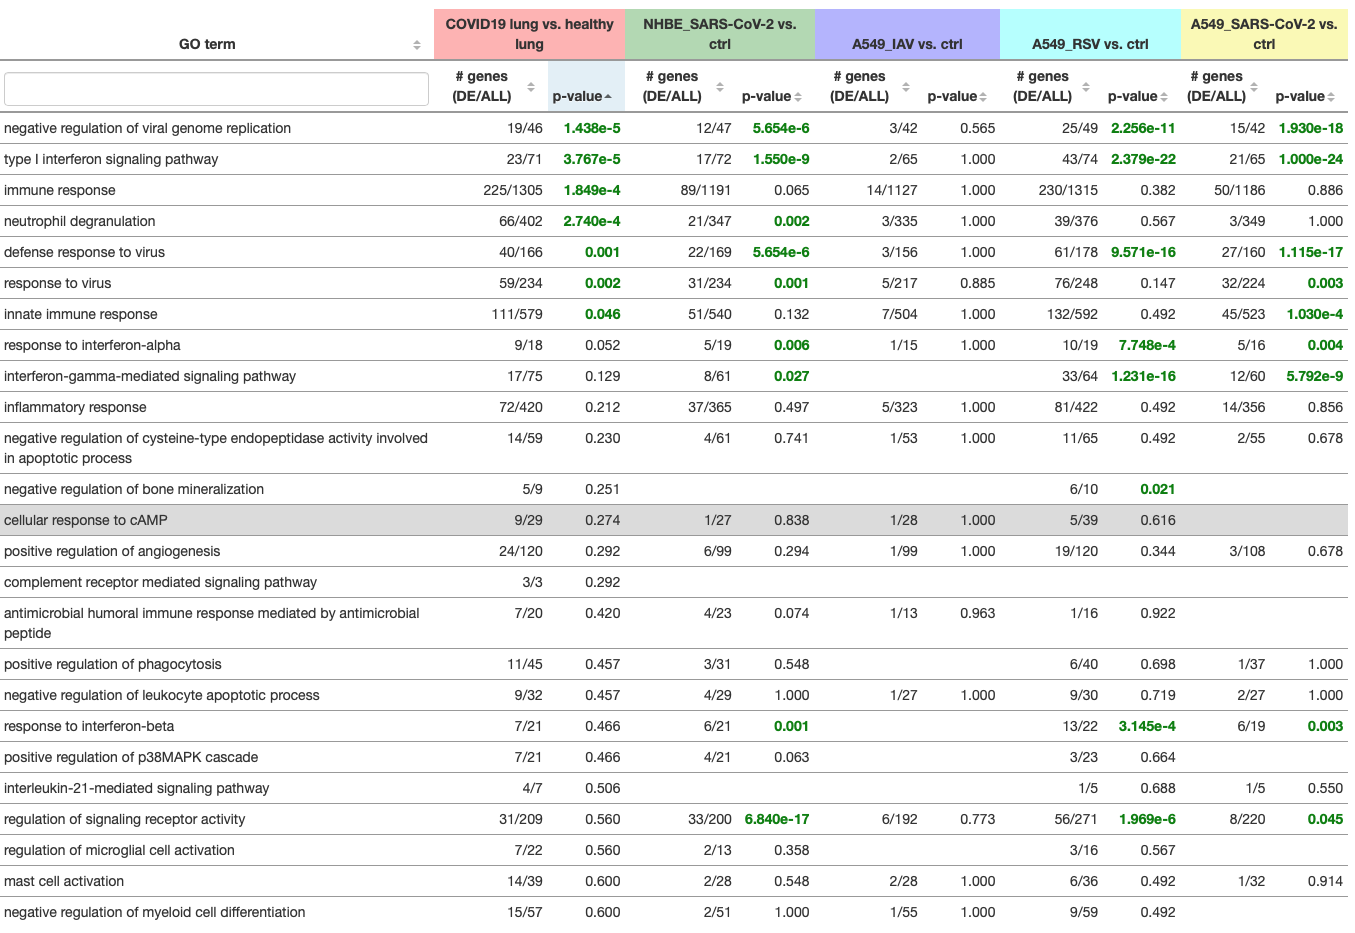
\includegraphics[width=1\linewidth]{../Figures/BPs_elim_FDR_all.png}
    \caption{Biological processes (BPs) identified as significant in the five experiments sorted by their significance in the COVID19vsControl. The  columns labelled ``\#genes'' show the number of differentially expressed (DE) genes out of the number of genes associated with the given biological process.  For instance for COVID19vsControl, the most significant BP is negative regulation of viral genome replication: 19 out of the 46 genes known to be involved in this process are differentially expressed and all but one of those are significantly up-regulated.  \label{Supp:BPs}}
        
\end{figure}

\begin{figure}
\centering
	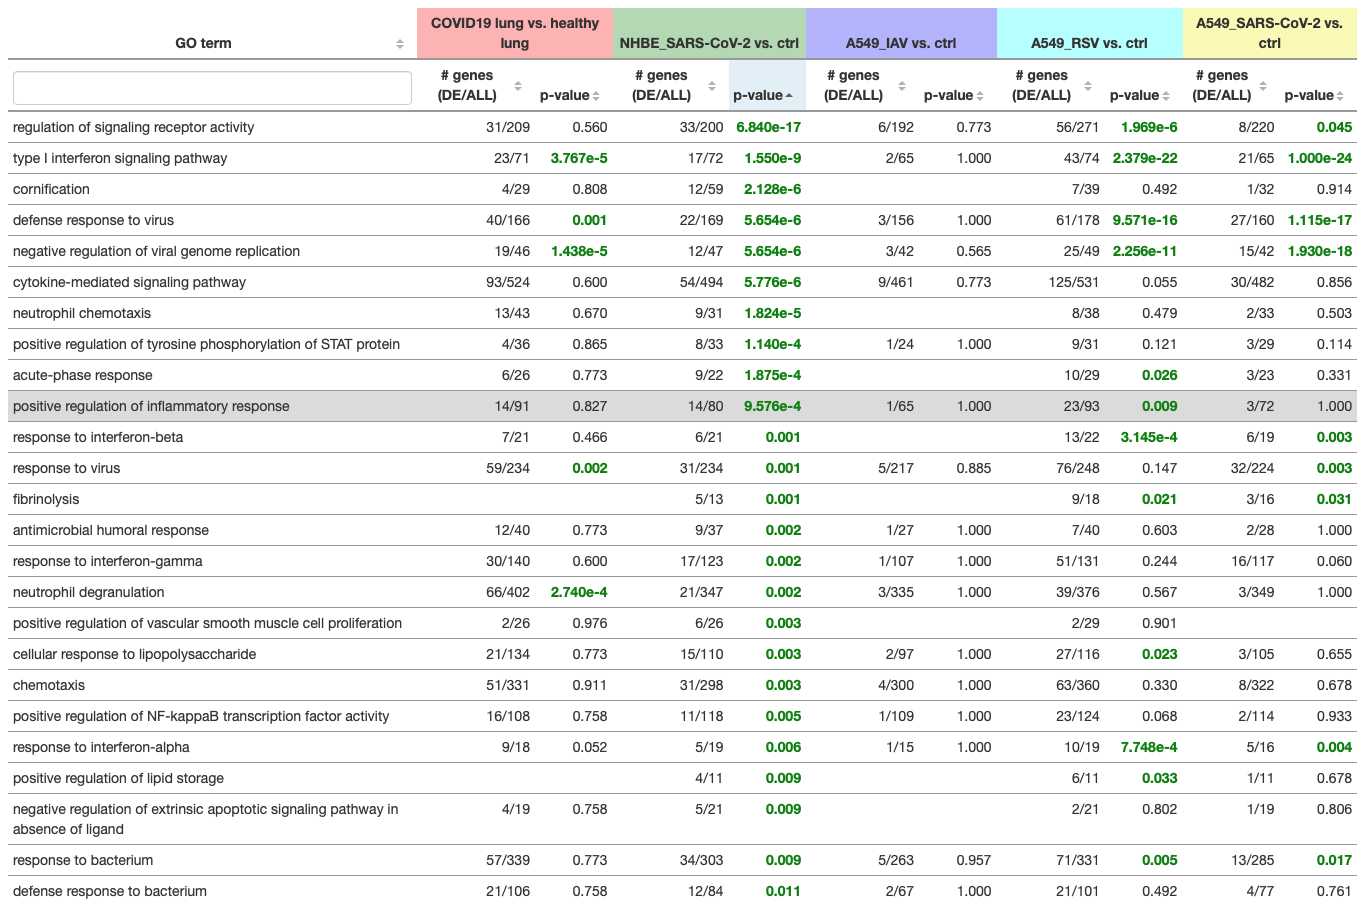
\includegraphics[width=1\linewidth]{../Figures/BPs_elim_FDR_all_orderedby_NHBE.png}
    \caption{Biological processes (BPs) identified as significant in the first five experiments sorted by their significance in NHBECoV2vsControl. The  columns labelled ``\#genes'' show the number of differentially expressed (DE) genes out of the number of genes associated with the given biological process. The p-values have been corrected with FDR. }
        \label{Supp:BP_orderedby_NHBE} 
\end{figure}


%\vspace{-3mm}
\subsubsection{Putative mechanisms of disease}

We performed an analysis aiming to identify putative mechanisms of  disease. As part of this analysis we identified four genes that were predicted to be activated upstream regulators based on the observed changes in their downstream genes. These were IRF9, STAT2, IFNG, and IFNB1. These suggest two different potential mechanisms. The first appears to be triggered by STAT2 and IRF9, which have 16 common target genes that are also all significantly up-regulated (IFI6, IFIT1, IFIT2, IFIT3, IFITM1, IFITM3, OAS1, OAS3, OAS S32, MX1, MX2, RSAD2, OASL, XAF1, IRF2, and IRF7). This mechanism is also known to be involved in the response to influenza A  (see  influenza A pathway in Fig.~\ref{Supp:influenzaA}). 

\begin{figure}
\centering
%	\includegraphics[width=0.8\linewidth]{influenza_A.png}
	\includegraphics[width=1\linewidth]{../Figures/influenza_A.png}
    \caption{The genes found to be differentially expressed in COVID-19 shown on the influenza A pathway. Note the putative mechanism triggered by STAT2 and IRF9 inferred from the SARS-CoV2 data is also present on the response to influenza A pathway shown here (rectangle).   Up-regulated genes are shown in shades of red, down-regulated genes are shown in shades of blue. OAS1, OAS2, OAS3 are grouped together as OAS downstream of IRF9. MX1 and MX2 are grouped together as MXA.  }
        \label{Supp:influenzaA} 
\end{figure}

The second putative mechanism involves interferon beta and gamma, which are targeting 5 common downstream genes: CXCL10, IDO1, DOX58, STAT1, which are up-regulated, and HMOX2 which is down-regulated. Interferon regulatory factors (IRFs) are subdivided into the interferonic IRFs (IRF2-3-7 and 9), the stress responsive IRFs (IRF1 and 5), the hematopoietic IRFs (IRF4 and 8) and morphogenic IRF6. IRF9 is a regulator of type I IFN signaling and is known to interact with STAT2~\cite{horvath1996interactions} and STAT1 to form the heterotrimeric transcription factor complex (ISGF3) that binds to interferon-stimulated response elements (ISREs) to induce the expression of interferon stimulated genes (ISG). During viral infections, ISGs perform two key functions: 1) directly limit viral replication by shutting down protein synthesis and triggering apoptosis; 2) activate key components of the innate and adaptive immune system, including antigen presentation and production of cytokines. The genes triggered by the STAT2 and IRF9 pathway include genes responsible for limiting viral replication (IFI6, IFIT1, IFIT2, IFIT3, IFITM1, IFITM3, OAS1, OAS3, OAS2, MX1, MX2, RSAD2, OASL) and inducers of apoptosis (XAF1, IRF2, IRF7). CXCL10, IDO1, DOX58, and STAT1 are genes associated with lymphocyte recruitment and immune regulation.


Interestingly, STAT2 and IRF9 together are also identified as activated upstream regulators due to 15 downstream targets even in the NHBECoV2vsControl (see Fig.~\ref{Supp:stat2irf9}). However, in the NHBE cells, the interferon activators were replaced by an interleukin based mechanism centered around IL1B, IL6, IL17A, adiponectin (ADIPOQ) and tumor necrosis factor (TNF).

\begin{figure}
\centering
%	\includegraphics[width=0.6\linewidth]{STAT2-IRF9.png}
	\includegraphics[width=1\linewidth]{../Figures/STAT2-IRF9.png}
    \caption{ STAT2  and IRF9 are identified as activated upstream regulators due to the 15 genes that are: i) immediately downstream of them, ii) differentially expressed and iii) consistent with their activation.  The colors represent the fold changes measured in COVID19vsControl. STAT2 is shown in gray because was measured to be up-regulated 2.265  fold, but its FDR-corrected p-value was not significant ($p=0.06$).}
        \label{Supp:stat2irf9}
\end{figure}

We also looked at genes that are known to modulate or inhibit the inflammatory response such as IL1RN IL10, and IL13. In the COVID19vsControl, IL1RN was up with a log2 fold change of 6.2 fold (a 78-fold increase, FDR-corrected $p=10^{-6}$),  IL10 was  up 2.8 fold (FDR-corrected $p=0.55$),  while the measurement for IL13 was not available.  In the NHBECoV2vsControl, IL1RN was up only 1.26 fold (FRD-corrected $p=0.035$), while measurements for IL10 and IL13 were not available. 
However, in this contrast, 14 out of 15 DE genes immediately downstream of IL10 and usually inhibited by IL10 were up-regulated which strongly supports the hypothesis that IL10 is inhibited (FDR-corrected $p=5.17\times 10^{-9}$). 



%\vspace{-5mm}
\subsubsection{Impacted pathways}

The significantly impacted  pathways are shown in Fig.~\ref{significant_pathways} and Fig.~\ref{Supp:pathways-meta_Bonferroni} ordered by their significance in COVID19vsControl and NHBECoV2vsControl, respectively. The p-values represent a combination of enrichment and perturbation p-values~\cite{DraghiciPE:2007} subsequently  corrected with FDR.  

\begin{figure}
\centering
%	\includegraphics[width=0.9\linewidth]{significant_pathways_FDR.png}
	\includegraphics[width=1\linewidth]{../Figures/significant_pathways_FDR.png}
    \caption{ The signaling pathways found to be significantly impacted in all five experiments ordered by their significance in the COVID19vsControl. The FDR-corrected p-values represent a combination of the p-value due to  enrichment and the p-value due to pathway impact. The column labelled ``\#genes'' shows the number of DE genes  and the total number of genes on each pathway. %\blue{\st{All p-values have been corrected for multiple comparisons wtih FDR}}. 
    }
        \label{significant_pathways}
\end{figure}

\begin{figure}
\centering
	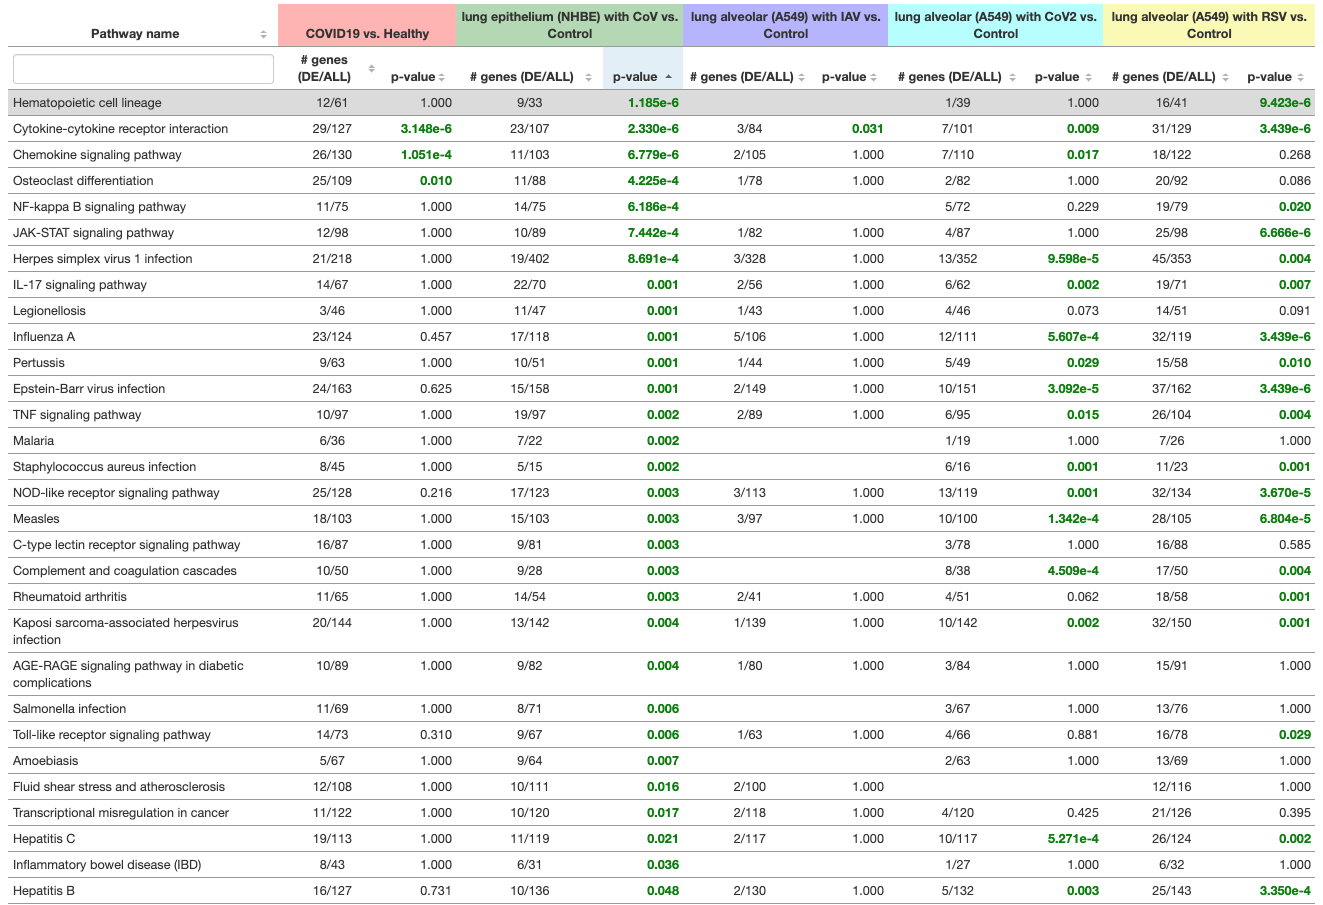
\includegraphics[width=1\linewidth]{../Figures/pathways-meta_Bonferroni.png}
    \caption{ The signaling pathways in all 5 experiments, ordered by their significance in NHBECoV2vsControl.  The Bonferroni-corrected p-values represent a combination of the p-value due to  enrichment and the p-value due to pathway impact. The middle column shows the number of DE genes  and the total number of genes on each pathway. 
    %\blue{\st{All p-values have been corrected for multiple comparisons with Bonferroni.}} 
    The most impacted pathway in NHBE is the hematopoietic pathway which may be linked to the hyper-coagulation phenomena observed in many COVID-19 patients. }
        \label{Supp:pathways-meta_Bonferroni}
\end{figure}

\begin{figure*}
\centering
	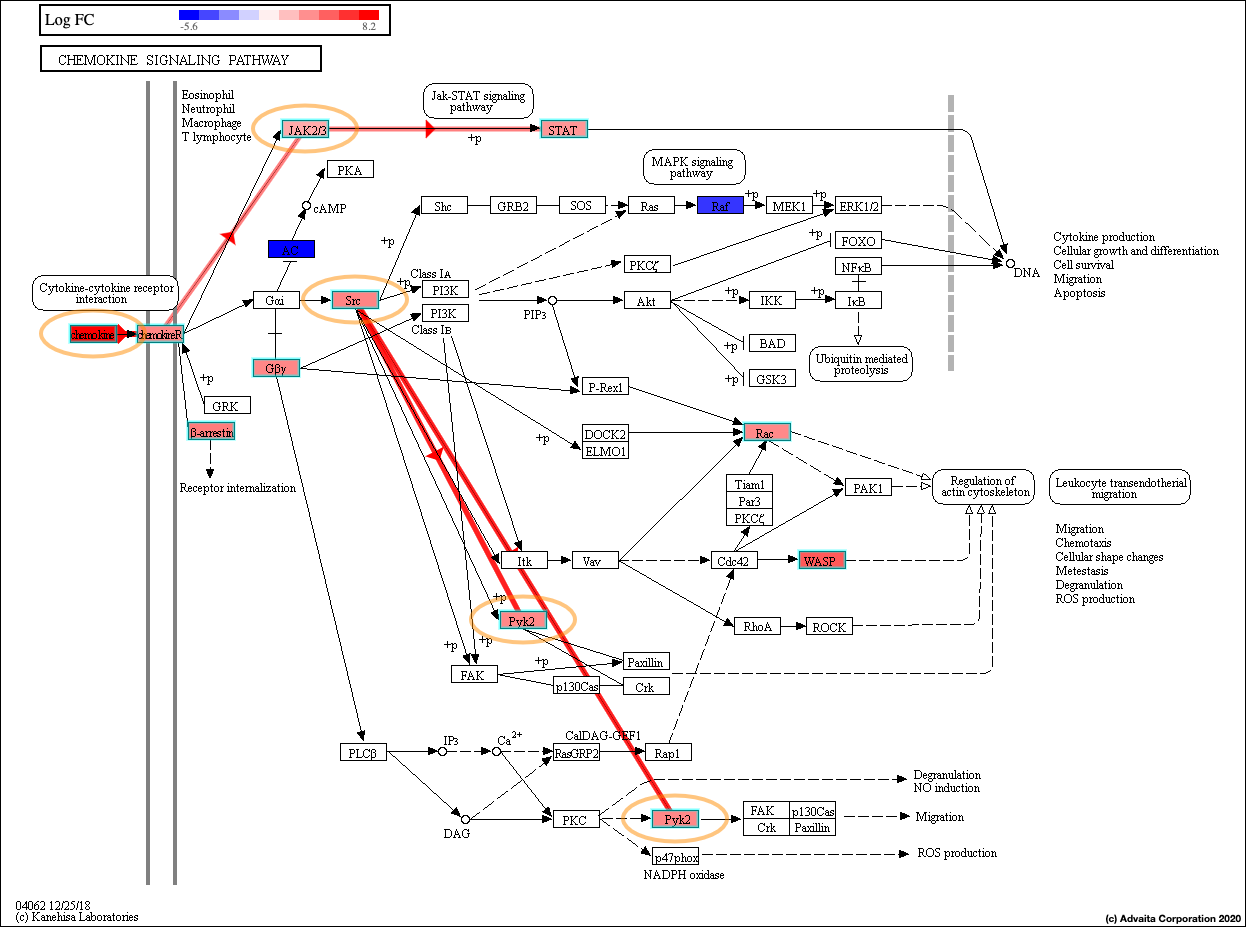
\includegraphics[width=0.9\linewidth]{../Figures/Chemokine_signaling_pathway.png}
    \caption{ The chemokine signaling pathway is the second most significantly impacted pathway in COVID19vsControl. The red arrows represent chains of coherent perturbation propagation, i.e. sequence of steps for which the observed expression changes are coherent with the expected changes according to the phenomena described by the pathway. The node labelled ``chemokines'' represents 11 chemokines measured to be up-regulated (CCL2, CCL3, CCL4, CCL7, CCL8, CCL11,  CCL18, CCL19, CXCL10, CXCL11, CXCL16 ). The CCR1 receptor is also up-regulated, as well as  JAK3 and STAT1. The ovals represent drug targets for which FDA-approved drugs already exist. 
    On this pathway, the impact is due both to the large number of DE genes  (26 out of 130), as well as to the signal propagation as shown by the red arrows. }
        \label{Supp:drugs_on_chemokine_signaling}
\end{figure*}

Fig.~\ref{Supp:cytokine-cytokine_pathway} shows the most impacted pathway, the \emph{Cytokine-cytokine interactions}. 
The gene expression changes on this pathway  show a very large number of pro-inflammatory cytokines and cytokine receptors being up-regulated, while several of the anti-inflammatory genes in the TGF-beta family are down-regulated. This corroborates the GO analysis finding above that there is a very strong positive regulation of inflammatory response. 
\color{black}



Fig.~\ref{Supp:drugs_on_chemokine_signaling} shows the \emph{Chemokine signaling pathway}.  
On this pathway, the impact is due both to the large number of DE genes (26 out of 130), as well as to the clear signal propagation from the chemokines outside the cell (11 chemokines up-regulated), through the chemokine receptor and via the JAK and STAT mechanism. 
Note that the same mechanism is also identified on the Influenza A pathway shown in Fig.~\ref{Supp:influenzaA}. \color{black}
Fig.~\ref{Supp:chemokine_signaling_mechanism} shows another view of the mechanism involving the genes on this pathway and all their known interactions.

\begin{figure}
\centering
	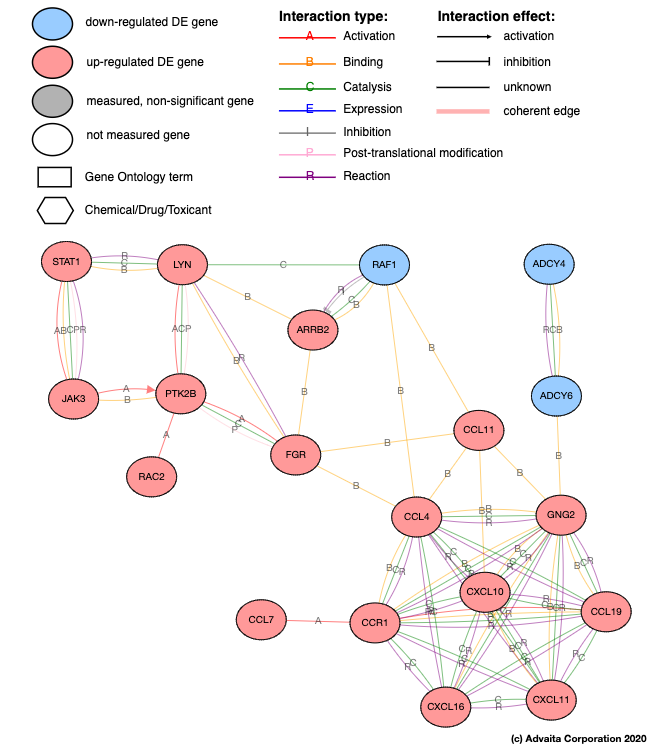
\includegraphics[width=0.8\linewidth]{../Figures/chemokine_signaling_mechanism.png}
    \caption{The known interactions involving the genes on the chemokine signaling pathway. }
        \label{Supp:chemokine_signaling_mechanism}
\end{figure}


Together, the GO analysis, pathway analysis and the putative mechanisms identified by the analysis above strongly  suggest a hyper-inflammation/cytokine storm.
\color{black} 


%\vspace{-3mm}
\subsubsection{Screening of potential therapeutic approaches: Proposed drugs}  

Once we identified the main regulatory pathways potentially associated with hyper-inflammation, we evaluated \emph{in silico} FDA-approved drugs that could show activity on multiple components of inflammation and consequently could be used for the management of severe COVID-19 cases. We considered the number of DE genes that would be reverted by each drug, as well as calculated a Bonferroni-corrected p-value indicating the suitability of each drug for repurposing in COVID-19 based on two different approaches (see ``Methods'' sub-section). We looked for drugs that have both small Benforroni-corrected p-values as well as revert a larger number of DE genes. 
The top five drugs drug identified by our analysis are shown in Fig.~\ref{top5drugs}. Methylprednisolone (MP) and prednisolone are corticosteroids currently used to modulate the immune response in rheumatoid arthritis.  Diclofenac is a non-steroidal anti-inflammatory drug (NSAID). Tofacitinib is a JAK inhibitor (see the JAK-STAT mechanism identified in  Fig.~\ref{Supp:drugs_on_chemokine_signaling}). Gold sodium thiomalate is an older anti-inflammatory drug, also used in the treatment of rheumatoid arthritis. 


 \textbf{Methylprednisolone} (MP) is the drug that was identified as the most likely to work by inhibiting the inflammatory pathway. This drug targets 27 genes that are found to be DE in COVID19vsControl. Out of these 27 genes, the drug would revert the changes in 25 of them. The drug also had an extremely significant p-value even after a Bonferroni correction which is the most stringent correction available ($p=5.72\times 10^{-10}$). MP also reverted 22 out of 22 genes found to be DE in NHBECoV2vsControl, and 25 out of 26 genes found to be DE in A549CoV2vsControl. 
Fig.~\ref{common_mechanism}  shows the putative mechanism through which MP acts on the DE genes in COVID19vsControl, and how these genes influence the BPs found to be significantly impacted.



%\vspace{-3mm}
\subsection{Validation on independent data sets}
The initial results obtained on from the data above were subsequently confirmed using additional data, spanning again all  three types of samples: cell lines, tissue cultures, and patient samples.   The additional cell line data include data from Vero E6 cells infected with SARS-CoV-2 vs. controls. Additional tissue cultures include lung organoids infected with SARS-CoV-2 vs. controls. In addition, even though the SARS-CoV-2 virus is primarily thought to infect the lungs with transmission through the respiratory route, it has been suggested that the intestine may present another viral target organ~\cite{Lamers:2020}. For this reason, we also compared the expression profiles of intestine organoids infected with SARS-CoV-2 vs. mock infection in differentiation and expansion media. These data are available in GEO as the GSE153940 (Vero E6 cells)~\cite{Riva:2020}, GSE160435 (lung organoids), and GSE149312 (intestinal organoids)~\cite{Lamers:2020} data sets. 

\begin{figure}
\centering
	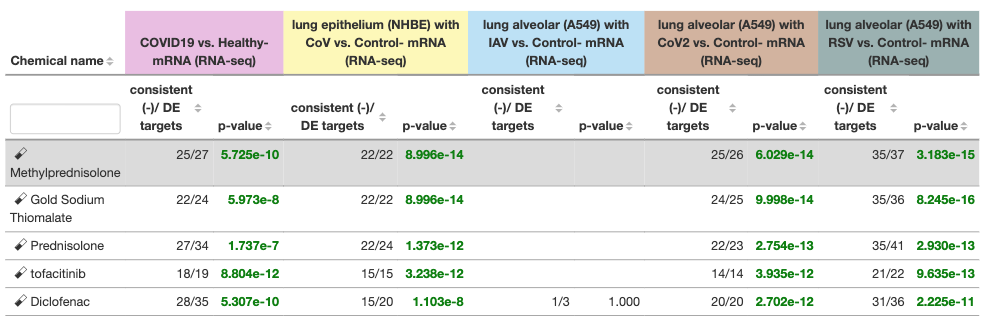
\includegraphics[width=1\linewidth]{../Figures/top5drugs.png}
    \caption{ The top five drugs proposed for repurposing. The table shows both p-values corrected with Bonferroni, as well as the number of DE genes that would be reverted out of the total number of  DE genes immediately downstream  of each drug (annotated as ``consistent (-)/DE targets" in the table).  Methylprednisolone (MP) and prednisolone are corticosteroids currently used to modulate the immune response in rheumatoid arthritis. Gold Sodium Thiomalate is an older drug, not currently in use in the US. Diclofenac is a NSAID and tofacitinib is a JAK inhibitor. The column for A549IAVvsControl is empty because there are no DE genes targeted by these drugs in this contrast.  }
        \label{top5drugs}
\end{figure} 

Finally, twenty nine additional samples from the lung of deceased COVID-19 patients with a high viral load and five controls were included from the Massachusetts General Hospital and Columbia University Irving Medical Center. These are available in GEO as the GSE150316 data set~\cite{desai2020temporal}.

 
Fig.~\ref{Supp:BPs_validation}  shows the biological processes common across the five additional independent data sets according to the the classical enrichment analysis. All of these are consistent with a viral response. In particular, the Type I interferon pathway is significant in every single data set analyzed, both initially, as well as in the additional validation data sets. The upstream regulators identified in the initial analysis, STAT2 and IRF9, were also found to be significant up-stream regulators in every single validation data set (see Fig.~\ref{Supp:STAT2-IRF9validation}).

\begin{figure}
\centering
	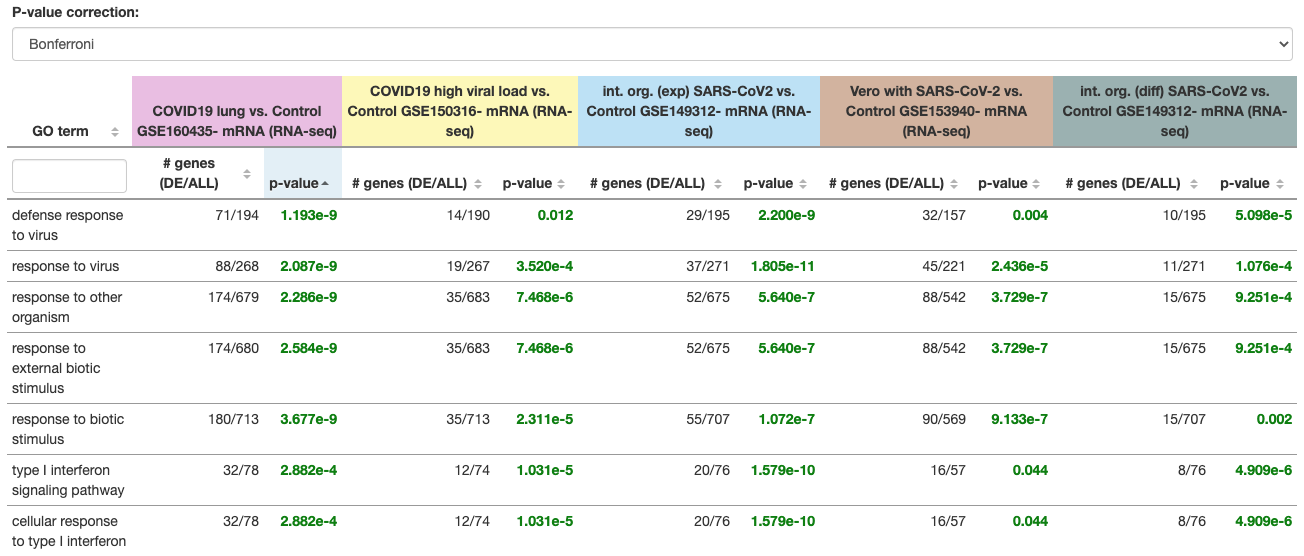
\includegraphics[width=1\linewidth]{../Figures/BPs_in_common_(Bonferroni)_in_additional_datasets.png}
    \caption{Biological processes (BPs) identified as significant in the additional independent data sets, as identified by a classical enrichment analysis. The  columns labelled ``\#genes'' show the number of DE genes out of the number of genes associated with the given biological process. The p-values have been corrected with Bonferroni. }
        \label{Supp:BPs_validation} 
\end{figure}

Fig.~\ref{Supp:drugs_validation} shows existing FDA-approved drugs identified as suitable candidates for repurposing based on these five additional data sets. These additional and independent data sets span across cell lines, cell cultures and patient data, as detailed above. Note that the top five drugs obtained on these additional data sets are matching perfectly with those shown in Fig.~\ref{top5drugs} even though the data sets analyzed were completely independent.

\begin{figure}
\centering
	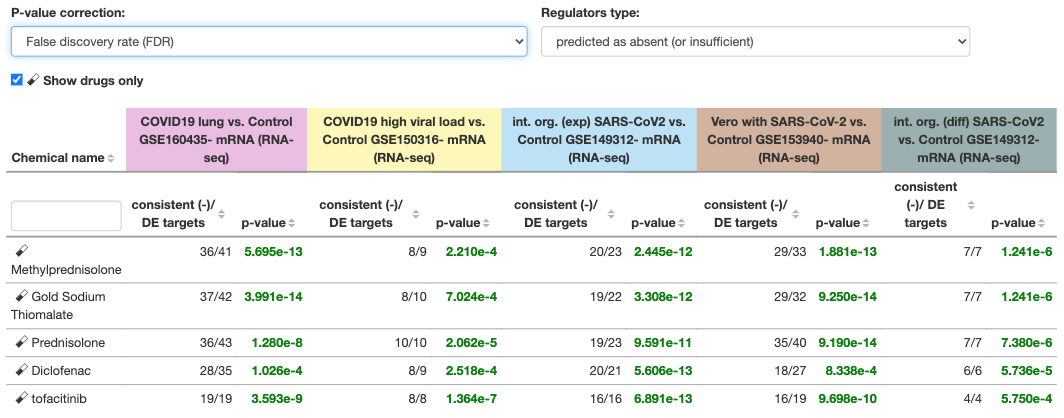
\includegraphics[width=1\linewidth]{../Figures/drugs_in_common_(Bonf)_validation.png}
    \caption{Existing FDA-approved drugs identified as suitable for the treatment of severe COVID-19 cases based on an additional five independent data sets. Note that the top five are identical with those shown in Fig.~\ref{top5drugs} even though the data sets analyzed were completely independent.}
        \label{Supp:drugs_validation}
\end{figure}

\begin{figure}
\centering
	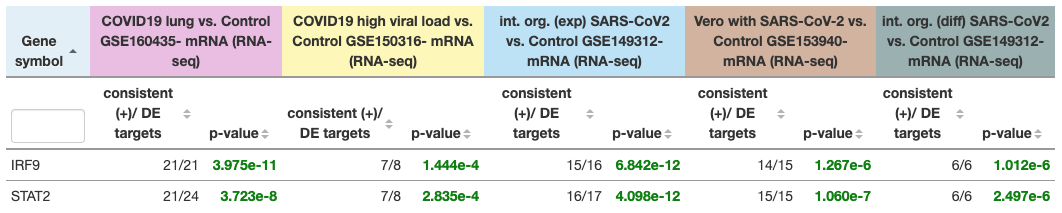
\includegraphics[width=1\linewidth]{../Figures/STAT2-IRF9validation.png}
    \caption{The STAT2 and IRF9 were found to be significant upstream regulators in all independent validation data sets. The p-values shown have been corrected with Bonferroni.}
        \label{Supp:STAT2-IRF9validation}
\end{figure}

%\color{black}
\subsection{In vivo effect of methylprednisolone: Clinical validation}

In an independent study, 213 patients diagnosed with COVID-19 were enrolled. 81 (38\%) received conventional therapy (control group) while 132 patients (62\%) received MP (MP group). The clinical characteristics and treatments received by the patients are shown in Table~\ref{Supp:clinicalcharacteristics} and Table~\ref{additionaltreatment}, respectively. As shown in Table ~\ref{endpoints}, thirty day all-cause mortality occurred at a significantly lower rate in the MP group compared to control group ($29.6\%$ vs. $16.6\%, p=0.027$). No statistical difference was detected in the proportion of patients prescribed empiric antibiotics or the time to empiric therapy. Kaplan Meier survival curve for 30-day mortality demonstrated increased probability of survival at 30-days in the MP group as compared to the control group ($p= 0.0204$) (Fig.~\ref{survival}).



\begin{table}
\footnotesize
\caption{Baseline Demographics and Clinical Characteristics of Study Patients }
\begin{center}
\begin{tabular}{p{7.5cm} cccc}
\hline
\textbf{Characteristics}  	&\makecell{\textbf{Total} \\ \textbf{(n=213)} }	& \makecell{\textbf{Pre-Protocol} \\ \textbf{(n=81)}} &	\makecell{\textbf{Post-Protocol}\\ \textbf{(n=132)}}	& \textbf{p-value}\\
\hline
\multicolumn{5}{l}{\textbf{Demographics}}\\
\hline
Age - median (IQR) - years &	62 (51-62)	 & 64 (51.5-3.5)	&61 (51-72)	& 0.400 \\
Male sex - no. (\%)	&109 (51.2)&	41 (50.6)	&68 (51.5)&	0.899\\
\multicolumn{5}{l}{Race}\\
\MyIndent Black - no. (\%)	&	155 (72.8)	&	50 (61.7)	&	105 (79.5)&	0.004\\
\MyIndent White - no. (\%) 	&	29 (13.6)	&18 (22.2)		&	11 (8.33)	&	0.005\\
Body mass index (IQR) - median (IQR) - kg/m$^{2}$	&32 (27.3-38.7)	&	30 (25-39)		&	33.2 (28.9-38.5)	&	0.007\\
\hline
\multicolumn{5}{l}{\textbf{Comorbidities } - no. (\%)}\\
\hline
Asthma &	33 (15.5)&	16 (19.8)	&17 (12.9)	&0.180\\
Chronic kidney disease  &	98 (46)	&41 (51.9)	&57 (43.5)&	0.240\\
Chronic obstructive pulmonary disease  &	27 (12.7)	&15 (18.5)	&12 (9.1)	&0.045\\
Congestive heart failure &	26 (12.2)	&10 (12.5)	&16 (12.2)&	0.951\\
Coronary artery disease &	38 (17.8)	&18 (22.2)	&20 (15.2)&	0.192\\
Diabetes	&105 (49.3)&	37 (45.7)	&68 (51.5)	&0.411\\
Hypertension& 	158 (74.2)	&62 (76.5)	&96 (72.7)	&0.925\\
Malignancy  	&24 (11.3)	&11 (13.6)	&13 (9.9)	&0.405\\
Smoking history  	&88 (41.3)&	40 (49.4)	&48 (36.4)&	0.0615\\
\hline
\multicolumn{5}{l}{\textbf{Presenting Symptoms}}\\
\hline
Cough - no. (\%)	&158 (74.2)	&62 (76.5)&	96 (72.7)	&0.536\\
Fever - no. (\%)	&150 (70.4)&	57 (70.4)	&93 (70.5)	&0.989\\
Myalgia - no. (\%)	&85 (39.9)&	32 (39.5)&	53 (40.2)	&0.926\\
Shortness of breath - no. (\%)	&148 (69.5)&	50 (61.7)	&98 (74.2)	&0.054\\
Duration of symptoms - median (IQR) - days&	5 (3-7)&	5 (2-7)&	6 (3-7)	&0.107\\
\hline
\multicolumn{5}{l}{\textbf{Severity of illness in emergency department (ED)}}\\
\hline
qSOFA - median (IQR)	&1 (0-1)	&1 (0-1)	&1 (0-1)	&0.850\\
NEWS - median (IQR)&	7 (4-10)	&7 (4-10)	&7 (4-9)	&0.668\\
Requiring mechanical ventilation in ED - no. (\%)	&22 (10.3)&	10 (12.3)&	12 (9.1)	&0.448\\
Direct admission to ICU - no. (\%)	&26 (12.2)&	11 (13.6)	&15 (11.4)&	0.631\\
\hline
\multicolumn{5}{l}{\makecell{*IQR denotes Interquartile range, NEWS denotes National Early Warning Score, qSOFA denotes quick Sequential\\ Organ Failure Assessment (qSOFA), ED denotes Emergency Department, ICU denotes intensive care unit} }\\
\end{tabular}
\end{center}
\label{Supp:clinicalcharacteristics}
\end{table}%

\begin{table}
\footnotesize
\caption{Treatments Received by Patients Pre-methylprednisolone and Methylprednisolone Protocol Groups}
\begin{center}
\begin{tabular}{p{7.5cm} cccc}
\hline
\textbf{Treatment} & 	\makecell{\textbf{Total} \\ \textbf{(n=213)}} &	\makecell{\textbf{Pre-Protocol} \\ \textbf{(n=81)}}	&\makecell{\textbf{Post-Protocol} \\ \textbf{(n=132)}}	& \textbf{p-value}\\
\hline
\multicolumn{5}{l}{\textbf{Antimicrobials}}\\
\hline
Empiric antibiotic prescribed for pneumonia -- no. (\%)	&163 (76.5)&	65 (80.2)	&98 (74)	&0.316\\
Time to empiric antibiotics - median (IQR) - days	&1 (0-1)&	1 (0-1)	&0 (0-1)	&0.631\\
Duration of antimicrobials - median (IQR) - days	&4 (2-5)	&5 (3-5)	&3 (2-5)	&0.009\\
Hydroxychloroquine use - no. (\%)	&161 (75.6)	&57 (70.4)&	104 (78.8)&	0.167\\
Time to hydroxychloroquine initiation - median (IQR) - days&	2 (1-3)	&3 (1-4)&	1 (0-2)&	0.126\\

Lopinavir/ritonavir and ribavirin use - no. (\%)&	10 (4.7)	&9 (11.1)	&1 (0.76)	&0.001\\
Remdesivir use -- no. (\%)	&5 (2.3)&	5 (6.2)	&0 (0)&	0.004\\
Tocilizumab use -- no. (\%)	&14 (6.6)&	8 (10.1)	&6 (4.5)	&0.126\\

\hline
\multicolumn{5}{l}{\textbf{Corticosteroid }}\\
\hline

Methylprednisolone received at any time - no. (\%)	&136 (63.8)&	46 (56.8)	&90 (68.2)	&0.094\\
Methylprednisolone received in first 48 hours - no. (\%)&	65 (30.5)	&10 (12.4)&	55 (41.7)	&$<$0.001\\
Time to steroid initiation from admission - median (IQR) - days &	2 (1-4)&	5 (3-7)	&2 (1-3)&	$<$0.001\\
Methylprednisolone dose - median (IQR) - mg	&40 (40-50)	&40 (40-50)&	40(35-50)	&0.851\\
Median duration of corticosteroids - median (IQR) - days&	3 (3-3)&	3 (3-3)&	3 (3-3)	&0.812\\


\hline

\multicolumn{5}{l}{*IQR denotes Interquartile range} \\
\end{tabular}

\end{center}
\label{additionaltreatment}
\end{table}%


\begin{table}
\footnotesize
\caption{Outcomes in the Pre-Corticosteroid and Corticosteroid Protocol Groups. CI denotes confidence interval, ICU denotes intensive care unit, GMU denotes general medical unit, ARDS denotes acute respiratory distress syndrome, IQR denotes Interquartile range. Note 1: A total of 10 and 12 patients were not included in this analysis because they required mechanical ventilation in the emergency department in the pre-corticosteroid and corticosteroid group, respectively. Note 2: A total of 11 and 15 patients were not included in this analysis because they were directly admitted to the intensive care unit in the pre-corticosteroid and corticosteroid group, respectively.}
\begin{center}
\begin{tabular}{p{6.5cm} cccc}
\hline
&\makecell{\textbf{Pre-Protocol}\\ \textbf{(n=81)}}	&\makecell{\textbf{Post-Protocol}\\ \textbf{(n=132)}}	&\textbf{Odds Ratio (CI)}	& \textbf{p-value}\\
\hline
\multicolumn{5}{c}{\textbf{Primary Outcome }}\\
\hline
30-day mortality - no. (\%)	& 24 (29.6)	& 22 (16.6)	&0.48 (0.25 - 0.92)	&0.027\\

\hline
%\multicolumn{5}{c}{\makecell{\footnotesize CI denotes confidence interval, ICU denotes intensive care unit, \\GMU denotes general medical unit, ARDS denotes acute respiratory distress syndrome, \\IQR denotes Interquartile range.}}\\
%\multicolumn{5}{c}{\makecell{\footnotesize }}\\
%\multicolumn{5}{c}{\makecell{\footnotesize }}
\end{tabular}
\end{center}
\label{endpoints}
\end{table}%


When comparing the two groups, those patients treated with a 3-day methylprednisolone protocol spent less time in the hospital (5 vs 8 days) and were less likely to be admitted to the ICU (27\% vs 44\%), being placed on a ventilator (22\% vs 37\%) or dying (14\% vs 26\%).

For a composite end point of preventing ICU admission, need for mechanical ventilator or mortality, the number needed to treat (NNT) to benefit a single patient was only 5 when methylprednisolone was used early in hospitalization. To prevent mortality, the NNT to benefit a single patient was only 8 for all hospitalized patients. This is in contrast to the RECOVERY trial (NCT04323592) for dexamethasone, where NNT was 8 for patients on mechanical ventilation and 25 for patients needed oxygen to prevent mortality.
\color{black}

\begin{figure}

	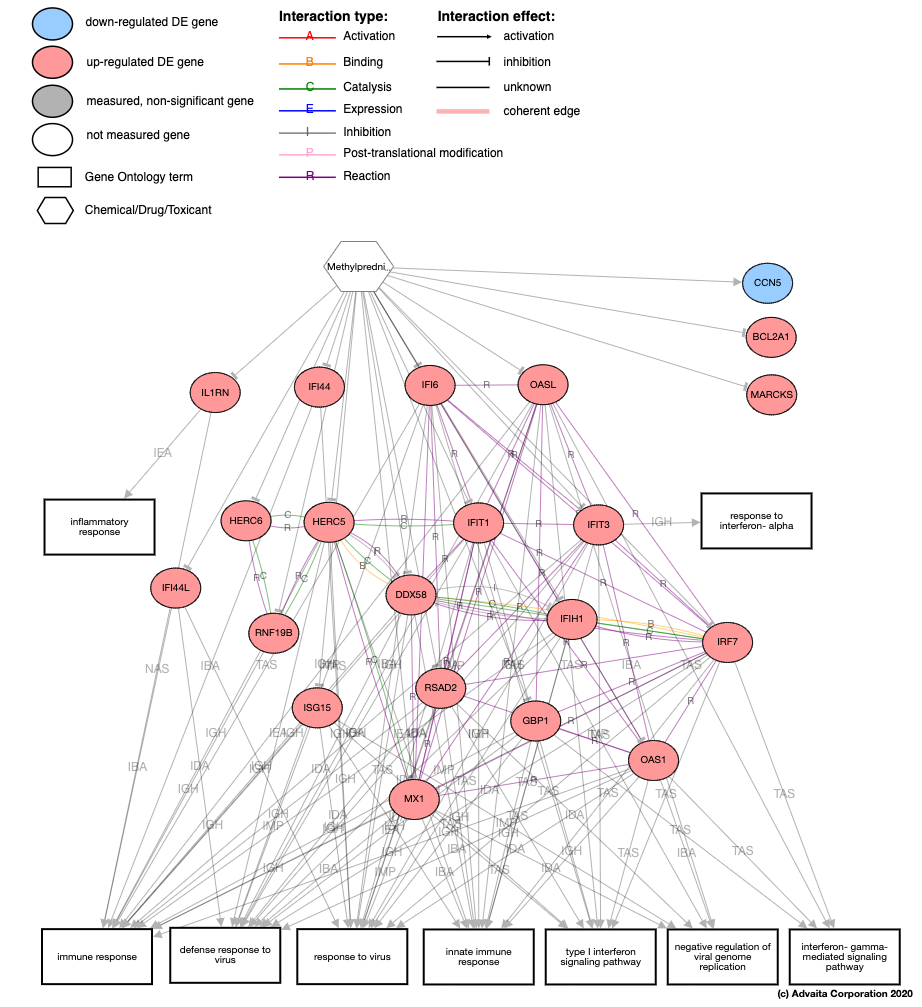
\includegraphics[width=1\linewidth]{../Figures/MethylprednisolonetoBPs.png}
         \caption{The putative mechanism through which MP acts on the genes measured to be DE, and  how these genes influence the  biological processes found to be significantly impacted in  the COVID19vsControl. This figure shows that: i) MP is known to revert the measured changes in all these 21 DE genes; ii) 20 out of these 21 DE genes are up-regulated suggesting a very strong immune response;  ii) many of the DE gene targeted directly by MP are directly involved in the top biological processes identified as significantly perturbed by the disease.} 
        \label{common_mechanism}
\end{figure}

%\vspace{-3mm}
\subsection{Other drugs investigated}

We also looked at other drugs that have already been proposed as repurposing candidates for COVID-19 including: \textbf{chloroquine}, \textbf{hydroxychloroquine}, \textbf{erythromycin},  \textbf{prednisone}, \textbf{dexamethasone},  \textbf{ibuprofen}, \textbf{ritonavir}, \textbf{aspirin}, and \textbf{clopidogrel}. Most or all of these drugs are currently under clinical trials~\cite{sanders2020pharmacologic}. 

\textbf{Chloroquine} was found to revert only 2 out of 4 genes found to be differentially expressed in the COVID19vsControl ($p=1$) and only 3 out of 6 genes found to be differentially expressed in NHBECoV2vsControl only ($p=1$). Furthermore, this drug was not found to be potentially effective in reversing the changes in A549RSVvsControl ($p=1$)  or A549CoV2vsControl ($p=1$). These results suggest that  chloroquine would not be a good potential candidate for repurposing for the goal of modulating the immune response.  

\textbf{Hydroxychloroquine}  did not appear as a good candidate for repurposing in any of the phenotypes and contrasts studied here. 
Chloroquine and hydroxychloroquine do not target any of the 21 genes that are both severely dysregulated, and also targeted by the proposed drugs. Note that while these drugs do not reverse observed gene expression changes, they may act as anti-virals by potentially inhibiting the viral replication~\cite{sanders2020pharmacologic}.

\textbf{Erythromycin}  targets only three DE genes in COVID19vsControl  and would revert only 2 of those. This yields an insignificant p value (Bonferroni-corrected $p=1$ and FDR-corrected $p=0.75$). 

\textbf{Ibuprofen} was also not found to be a good candidate for use in COVID-19, having the potential to revert only 4 out of 10 DE genes ($p=1$). This suggests a  phenomenon in the class of NSAIDs similar with that observed within the corticosteroids: while one or two specific drugs may be effective, 
these effects cannot be generalized to the entire class. 
In other words, not all NSAIDs may be equally helpful in modulating the over-inflammation induced by COVID-19. 

\textbf{Ritonavir} was found to be significant ($p=0.002$) in reverting changes in 8 out of its 10 targets that were measured to be differentially expressed in NHBECoV2vsControl. However, ritonavir was not found to be effective in reversing the gene changes induced in COVID19vsControl.

\textbf{Clopidogrel} targets only one DE gene in COVID19vsControl, one DE gene in A549CoV2vsControl, and no DE gene in NHBECoV2vsControl. These results suggest that this drug is unlikely to be effective in COVID-19 with a p-value of 1 across all experiments. 
 
 Finally, \textbf{aspirin}  is targeting 44  DE genes in COVID19vsControl but  reversing only 22 of them. In NHBECoV2vsControl samples, aspirin was found to target 18 genes and revert 12 on them. In NHBE, aspirin has a raw p-value of 0.028 but after an FDR correction this becomes 0.187. In the COVID19vsControl contrast, even the raw p-value is 0.939 and  becomes 1 after any correction. 
 
\begin{figure}
\centering
	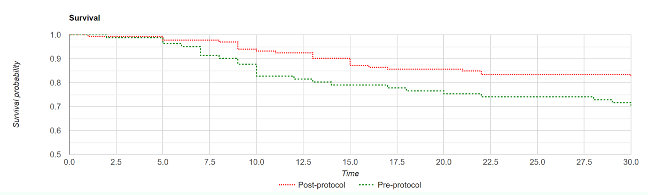
\includegraphics[width=1\linewidth]{../Figures/Survival_methylprednisolone.png}
        \caption{Kaplan Meier survival curve for 30-day mortality demonstrating increased probability of survival at 30-days in the post methylprednisolone cohort as compared to the pre-methylprednisolone cohort (p= 0.0204).  }
        \label{survival}
\end{figure}



%\vspace
\subsection{Discussion}

In the present study we described an initial characterization of the main pro-inflammatory pathways induced by SARS-Cov-2 infection on human lung epithelial cells and the identification of the most effective therapeutic approach to inhibit this cytokine storm.


In this study we have identified MP as the most effective, FDA approved, drug that targets critical components of the inflammatory pathway responsible for ARDS.  Furthermore, we demonstrated its efficacy  in a clinical trial in which MP decreased the incidence of mortality in COVID-19 patients. An important finding of this study is that drugs in the same class might not necessarily have similar effects. For instance, MP and prednisolone were predicted to be effective in reverting many of the changes triggered by COVID-19, while other closely-related corticosteroids such as prednisone were not. MP and prednisolone are corticosteroids currently used to modulate the immune response in rheumatoid arthritis. Interestingly, we observed that the putative mechanisms through which these drugs would revert the genes dysregulated in COVID-19 are different (Fig.~\ref{both_mechanisms}). MP for example inhibits STAT1, IFT3 and HERC5 while prednisolone has an impact on IFIT genes such as IFT1, IFIT3, IFI6, and IFI4L.

We also looked at other corticosteroids such as prednisone, and hydrocortisone. However, prednisone was found to target only 3 DE genes in the COVID19vsControl and only 2 DE genes in the NHBECoV2vsControl. From those, prednisone would revert only 1 of the 3 DE genes in the COVID19vsControl and 0 out of 2 DE genes in the NHBECoV2vsControl. Both yielded insignificant Bonferroni-corrected p-values ($p=1$) suggesting that prednisone is not expected to be a highly effective treatment. Prednisolone, dexamethasone, and hydrocortisone belong to the same family of corticosteroid anti-inflammatory agents and there is also a structural similarity between them (Fig.~\ref{Supp:steroids}). In spite of this structural similarity, hydrocortisone is known to revert only 8 out of 10 DE genes in the COVID19vsControl (FDR-corrected $p=0.57$) and 5 out of 8 DE genes in the NHBECoV2vsControl (FDR-corrected $p=0.038$, Bonferroni-corrected  $p=1$). Dexamethasone was found to revert 33 out of 69 DE genes in the COVID19vsControl (FDR-corrected $p=1$) and 27 out of 45 DE genes in the NHBECoV2vsControl (FDR-corrected $p=0.002$, Bonferroni-corrected $p=0.066$). Dexamethasone is significant in the NHBECoV2vsControl but not in the COVID19vsControl. Hydrocortisone appears as significant in COVID19vsControl, but only marginally so in the NHBECoV2vsControl.

\begin{figure}
\centering
	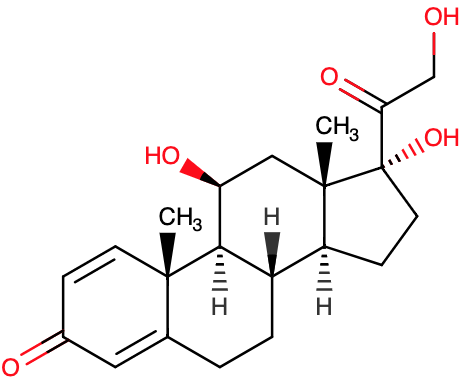
\includegraphics[width=0.2\linewidth]{../Figures/prednisolone.png}
	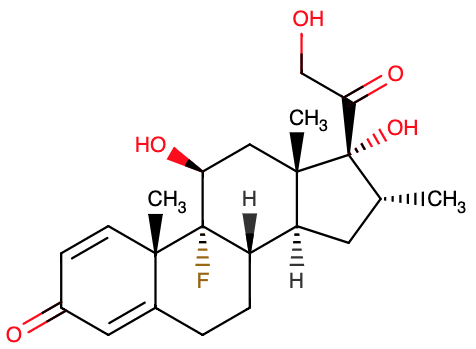
\includegraphics[width=0.2\linewidth]{../Figures/dexamethasone.png}
	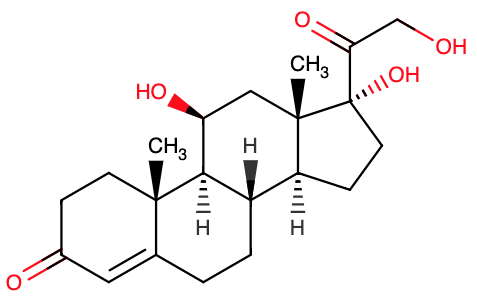
\includegraphics[width=0.2\linewidth]{../Figures/hydrocortisone.png}
        \caption{Three closely related steroidal anti-inflammatory: prednisolone, dexamethasone, and hydrocortisone. However, the results shown here suggest that prednisolone would have the highest impact on the genes dis-regulated in COVID-19, followed by dexamethasone. Currently available data suggest that hydrocortisone and prednisone would not revert many of the DE genes dis-regulated by COVID-19.}
        \label{Supp:steroids}
\end{figure}

Such differences between drugs in the same class can be potentially explained in two ways. First, different drugs can be associated with a different number of annotations. For instance, the number of genes that a given drug is known to be targeting can influence its significance. Table~\ref{Supp:drugcoverage} shows the number of known targets associated with some drugs relevant to COVID-19. Second, there could be genuine differences between the effectiveness of different corticosteroids, potentially due to a different number of genes truly impacted by each drug. The results of these study, based on all annotations available to date, suggest that MP would revert the largest number of the gene perturbed by COVID-19, followed by dexamethasone and, as shown in the outcome of COVID-19 infected patients, have a major impact on their clinical outcome. Prednisone and hydrocortisone revert much fewer known genes and consequently, could have an effect but it is expected to be less effective than the one observed with MP.  Future clinical trials comparing the efficacy of these different corticosteroids are necessary to confirm our findings


\begin{table}
\footnotesize
\caption{The quality of the coverage in the annotations used. The first column shows the number of edges  corresponding to increased or decreased expression induced by each drug considered. Each edge corresponds to a gene that is known to be affected by the given drug. Note that larger numbers increase the probability that a drug would target more of the genes impacted by the disease, but do not necessarily stand for higher predicted efficacy.  The second column shows the number of these targets found to be differentially expressed (DE) in COVID19vsControl. Finally, the third column shows the number of such DE targets that are expected to be reversed by the drug based on existing knowledge and annotations. }
\begin{center}
\begin{tabular}{lc>{\centering\arraybackslash}p{30mm}>{\centering\arraybackslash}p{34mm}}
\hline
Drug 		  & known drug targets interactions &  targets changed by SARS-COV-2 (DE) & DE  targets reverted by the drug \\ \hline
Dexamethasone & 958 		    & \makecell[c]{69}  & \makecell[c]{33} \\
Aspirin  		  &448 		    & \makecell[c]{44}  & \makecell[c]{22} \\
Ibuprofen & 135 &  \makecell[c]{10} & \makecell[c]{4} \\
Prednisolone & 119 &  \makecell[c]{34} & \makecell[c]{27} \\
Methylprednisolone & 85 &  \makecell[c]{27} & \makecell[c]{25}\\
Ritonavir		  &	73 & \makecell[c]{10} & \makecell[c]{9}\\
Chloroquine & 33 & \makecell[c]{4} & \makecell[c]{2} \\
Erythromycin& 19 &  \makecell[c]{3} & \makecell[c]{2} \\
Prednisone & 16&  \makecell[c]{3}& \makecell[c]{1}\\
Clopidogrel & 7 &  \makecell[c]{1} & \makecell[c]{0}\\
Hydroxychloroquine & 6 & \makecell[c]{1} & \makecell[c]{0} \\
\hline
\end{tabular}
\end{center}

\label{Supp:drugcoverage}
\end{table}%

The host inflammatory response in the lungs lead to acute lung injury and ARDS. This constitutes the main rationale for the use of corticosteroids. However, administration of corticosteroids is associated with multiple side effects, such as an increased risk of secondary infection and delayed viral clearance. A recent article in Lancet reports that clinical evidence does not support corticosteroid treatment for COVID-19~\cite{russell2020clinical}. However, this report looks at corticosteroids as an entire class of drugs. A recent retrospective study of 201 patients with COVID-19 in China found that treatment with MP for those who developed ARDS was associated effective in decreasing the risk of death. Among patients with ARDS, treatment with MP decreased the risk of death (HR, 0.38; 95\% CI, 0.20-0.72). In this study, 23 of 50 [46\%] patients with MP treatment died compared to 21 deaths out of  34 patients without MP treatment~\cite{wu2020risk}. Both reports are entirely consistent with our findings: corticosteroids in general are NOT expected to help as a class of drugs, but rather each steroid should be assessed individually.


Methylprednisolone has been also the focus on several other recent clinical studies. Wu \emph{et al.} studied the effect of MP  in a cohort of 201 COVID-19 patients, of which 84 developed ARDS~\cite{WuRiskFactorsCOVID:2020}.  They report that ``among patients with ARDS, treatment with MP decreased the risk of death (HR, 0.38; 95\% CI, 0.20-0.72).'' The percentage of people who developed ARDS and eventually died was reduced from  61.8\% (21 of 34) to 46\% (23 of 50).

Salton \emph{et al.}  conducted a multi-center, observational study to explore the association between a prolonged, low-dose of MP and a composite endpoint including the need for ICU referrals, intubation, or death within 28 days (\href{www.clinicaltrials.gov}{www.clinicaltrials.gov}, NCT04323592)~\cite{salton2020prolonged}. They found that in a cohort of 83 patients treated with MP and 90 controls, the treatment with MP significantly lowered the hazard of death (71\%). The composite end point was met by 19 vs. 40 (adjusted hazard ratio (HR) 0.41; 95\% confidence interval (CI): 0.24-0.72). Transfer to ICU and need for invasive MV was necessary in 15 vs. 27 ($p=0.07$) and 14 vs. 26 ($p=0.10$), respectively. By day 28, the MP group had fewer deaths (6 vs. 21, adjusted HR=0.29; 95\% CI: 0.12-0.73) and more days off invasive MV (24.0 +/- 9.0 vs. 17.5 +/- 12.8; $p=0.001$).

\begin{figure}
\centering
	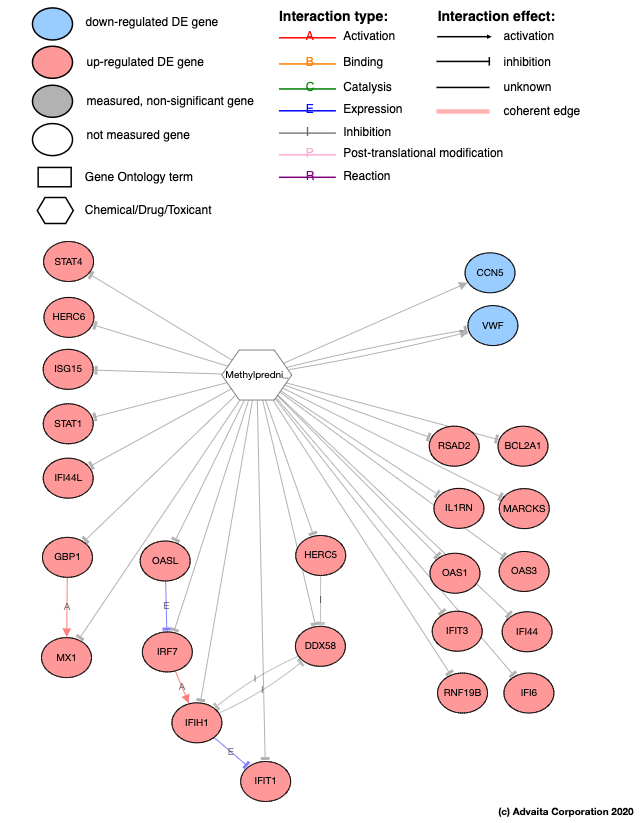
\includegraphics[width=0.8\linewidth]{../Figures/Methylprednisolone_mechanism.png}
        \caption{The putative mechanisms through which methylprednisolone  would revert the  changes triggered by COVID-19  in the lung tissue.}
        \label{both_mechanisms}
\end{figure}

A similar multi-center study focus on MP was undertaken in Spain (European Clinical Trials Register: 2020-001934-37). This study involved 85 patients of which 34 were randomized to MP, 22 were assigned to MP by the clinician and 29 constituted the control group. The composite endpoint requirement of non-invasive ventilation, admission to ICU, and death. This study reported that the use of MP was associated with a reduced risk of the composite endpoint  (RR 0.55 95\% CI 0.33-0.91) ({https://www.medrxiv.org/content/\\10.1101/2020.06.17.20133579v1}).

Finally, preliminary results from a large randomized study undertaken in the UK \\(NCT04381936) show that dexamethasone is also able to significantly reduce the number of deaths. In this study the steroid group included 2,100 participants and was compared with the standard of care group including 4,300 participants. Unfortunately, this study placed dexamethasone in the same arm with MP (MP to be administered to pregnant women instead of dexamethasone), so this study will not be able to elucidate whether MP and dexamethasone have any differences in efficacy. However, the results of the clinical study presented here suggest that MP has a lower NNT than dexamethasone. The potential higher efficacy of MP needs to be confirmed in larger cohorts. However, in a recent meta-analysis of randomized studies investigating prolonged corticosteroid treatment in non-viral ARDS, methylprednisolone treatment achieved a reduction in duration of mechanical ventilation and mortality superior to that of dexamethasone or hydrocortisone~\cite{meduri2020pharmacological}.

We also looked at other drugs that have already been proposed as repurposing candidates for COVID-19 including: chloroquine, hydroxychloroquine, erythromycin, prednisone, ibuprofen, ritonavir, aspirin, and clopidogrel. None of these was predicted to be effective in reverting SARS-CoV2 gene expression changes (see Table ~\ref{Supp:drugcoverage}).

\begin{table}
\small
\begin{center}
\begin{tabular}{l||c|>{\centering\arraybackslash}p{30mm}|>{\centering\arraybackslash}p{34mm}}
\hline
Drug 		  & known drug targets interactions &  targets changed by SARS-COV-2 (DE) & DE  targets reverted by the drug \\ \hline
Dexamethasone & 958 		    & \makecell[c]{69}  & \makecell[c]{33} \\
Aspirin  		  &448 		    & \makecell[c]{44}  & \makecell[c]{22} \\
Ibuprofen & 135 &  \makecell[c]{10} & \makecell[c]{4} \\
Prednisolone & 119 &  \makecell[c]{34} & \makecell[c]{27} \\
Methylprednisolone & 85 &  \makecell[c]{27} & \makecell[c]{25}\\
Ritonavir		  &	73 & \makecell[c]{10} & \makecell[c]{9}\\
Chloroquine & 33 & \makecell[c]{4} & \makecell[c]{2} \\
Erythromycin& 19 &  \makecell[c]{3} & \makecell[c]{2} \\
Prednisone & 16&  \makecell[c]{3}& \makecell[c]{1}\\
Clopidogrel & 7 &  \makecell[c]{1} & \makecell[c]{0}\\
Hydroxychloroquine & 6 & \makecell[c]{1} & \makecell[c]{0} \\
\hline
\end{tabular}
\end{center}
\caption{The quality of the coverage in the annotations used. The first column shows the number of edges  corresponding to increased or decreased expression induced by each drug considered. Each edge corresponds to a gene that is known to be affected by the given drug. Note that larger numbers increase the probability that a drug would target more of the genes impacted by the disease, but do not necessarily stand for higher predicted efficacy.  The second column shows the number of these targets found to be differentially expressed (DE) in COVID19vsControl. Finally, the third column shows the number of such DE targets that are expected to be reversed by the drug based on existing knowledge and annotations. }
\label{Supp:drugcoverage}
\end{table}%
 
In summary, we describe the inflammatory pathways associated with the cytokine storm found in COVID-19 patients and describe the characterization of the potential effective therapeutic approaches that, by targeting these pathways could effectible reduce the hyper-inflammatory response responsible for the development of ARDS, a main cause of mortality in COVID-19 patients.  Clinical results confirmed the efficacy of the \emph{in silico} prediction that indicated MP could improve outcomes in severe COVID-19. 



%\vspace{-5mm}
\subsection{Methods}
\textbf{Gene Ontology (GO) analysis method.}  For each GO term~\cite{ashburner2002ontologies, gene2004gene}, the number of differentially expressed (DE) genes annotated to the term is compared to the number of DE genes expected just by chance. We used  an over-representation approach to compute the statistical significance of observing at least the given number of DE genes, as proposed by~\cite{Tavazoie:1999}. The uncorrected p-value is computed using the hypergeometric distribution, as previously described~\cite{DraghiciOE2:2003, DraghiciBook:2011}, and corrected with FDR and Bonferroni.

The classical method used above considers all GO terms to be independent. However, given the nature of gene ontology, considering the genes multiple times introduces errors~\cite{Rhee:2008, DraghiciBook:2011}. Due to the ``true path rule'', all  genes annotated to a GO term are also annotated to all its ancestors when traversing ``is a'' relationships. Because of this, the same genes are counted in the enrichment of every term above the one they are directly annotated with.  We used an approach inspired by  the \textit{elim} and \emph{weight} pruning methods as originally proposed by Alexa \textit{et al.}~\cite{Alexa:2006}. The algorithm constructs a custom cut through the GO hierarchy by starting with the most specific nodes and calculating their uncorrected p-value with all genes assigned directly to each such node. If a node is significant, it is reported as such. If the node is not significant, the genes associated to the given node are propagated to its direct ancestors and a uncorrected p-value is calculated for each of those. 

\textbf{Pathway analysis method.}  
iPathwayGuide (\url{www.advaitabio.com}) assesses pathways using the Impact Analysis method as previously published~\cite{DraghiciPE:2007, tarca2009novel, khatri2007}. The impact analysis uses two types of evidence: i) the over-representation of differentially expressed (DE) genes in a given pathway and ii) the perturbation of that pathway computed by propagating the measured expression changes across the pathway topology. These aspects are captured by two independent probability values, $pORA$ and $pAcc$, that are then combined in a unique pathway-specific uncorrected p-value. The underlying pathway topologies, comprised of genes and their directional interactions, are obtained from the KEGG database~\cite{ogata1999kegg, kanehisa2010kegg, kanehisa2012kegg,  kanehisa2014data}.

The first probability, $pORA$, expresses the probability of observing the number of DE genes in a given pathway that is greater than or equal to the number observed, by random chance~\cite{DraghiciOE2:2003,DraghiciBook:2011}. Let us consider there are $N$ genes measured in the experiment, with $K$ of these on the given pathway. Based on the user-defined a priori selection of DE genes, $n$ out of $N$ genes were found to be differentially expressed. The probability of observing exactly $k$ differentially expressed genes on the given pathway is computed based on the hypergeometric distribution.

Because the hypergeometric distribution is discrete, the probability of observing fewer than $k$ or more genes on the given pathway just by chance is defined as 1 minus  the hypergeometric cumulative density function evaluated at $k-1$.


The second probability, $pAcc$, is calculated based on the amount of total accumulation measured in each pathway. A perturbation factor is computed for each gene on the pathway using:

\begin{equation}
\label{eqn:PF}
PF(g) = \alpha(g) \cdot \Delta E(g) + \sum_{u \in US_g} \beta_{ug}\frac{PF(u)}{N_{ds}(u)}
\end{equation}


In Equation~\ref{eqn:PF}, $PF(g)$ is the perturbation factor for gene $g$, the term $\Delta E(g)$ represents the observed fold change of gene $g$, and $\alpha(g)$ is an a priori weight that can be used to incorporate information about the type of gene or its significance~\cite{voichita2012incorporating}. In this analysis, all gene were treated equally (all $\alpha(g)=1$). The last term is the sum of the perturbation factors of all genes $u$, directly upstream of the target gene $g$, normalized by the number of downstream genes of each such gene $N_{ds}(u)$. The value of $\beta_{ug}$ quantifies the strength of the interaction between genes $g$ and $u$. The sign of $\beta$ represents the type of interaction: positive for activation-like signals, and negative for inhibition-like signals. Subsequently, iPathwayGuide calculates the accumulation at the level of each gene, $Acc(g)$, as the difference between the perturbation factor $PF(g)$ and the observed fold change:

\begin{equation}
Acc(g) = PF(g) - \Delta E(g)
\label{eqn:acc}
\end{equation}

All perturbation accumulations are computed at the same time by solving the system of linear equations resulting from combining Equation~\ref{eqn:PF} for all genes on a given pathway. Once all gene perturbation accumulations are computed, iPathwayGuide computes the total accumulation of the pathway as the sum of all absolute accumulations of the genes in a given pathway. The significance of obtaining a total accumulation ($pAcc$) at least as large as observed, just by chance, is assessed through bootstrap analysis.

The two types of evidence, $pORA$ and $pAcc$, are combined into an overall pathway score by calculating an uncorrected p-value using Fisher's method. This p-value is then corrected for multiple comparisons using false discovery rate (FDR)~\cite{Benjamini:1995,  Benjamini:2001} and Bonferroni~\cite{Bonferroni:1935} corrections. 


The underlying pathway topologies, comprised of genes and their directional interactions, are obtained from the KEGG database~\cite{ogata1999kegg, kanehisa2010kegg, kanehisa2012kegg,  kanehisa2014data}.


\textbf{Putative mechanism inference.} The impact analysis  allows the computation of the perturbation at the level of every gene on every pathway. Putative mechanisms are identified as sequences of pathway signals for which the measured gene expression changes are consistent with the sequence of events described by the pathway. An example would be the chemokine-chemokine receptor-JAK-STAT sequence identified on the Chemokine Signaling Pathway  in Fig.~\ref{Supp:drugs_on_chemokine_signaling}. This approach is able to identify candidates for potentially active mechanisms on existing pathways and has also been shown to have an increased accuracy~\cite{nguyen2019identifying}. %In order to 


\textbf{The prediction of upstream Chemicals, Drugs, Toxicants (CDTs)} is based on two types of information: i) the enrichment of DE genes from the experiment and ii) a network of interactions from the Advaita Knowledge Base (AKB v1910). The network is a directed graph in which the source node represents either a chemical substance or compound, a drug, or a toxicant (CDT). We focused our work on FDA-approved drugs that could be repurposed. The edges represent known effects that these CDTs have on various genes. A signed edge in this graph consists of a source CDT ($u$), a target gene, and a sign to indicate the type of effect: activation ($+1$) or inhibition ($-1$). 
The variable $u$ here stands for a CTD but its role is similar to the role of the upstream gene as used in Equation~\ref{eqn:PF} in the impact analysis. In both cases, the analysis is performed on a graph in which ``u'' is the immediately upstream node. In the impact analysis, the upstream node was  a gene whereas here, the upstream node will represent a CTD.

The analysis considers the hypothesis that  the upstream chemical, drug or toxicant is absent (or insufficient) in the condition studied. In essence, a drug for which this hypothesis is supported by a significant amount of evidence will be a very strong candidate for repurposing because such drug will effectively reverse many of the gene expression changes observed in the given disease. 


The analysis divides the set of all the genes from the AKB into several subsets based on the measurements in the experiment and the definitions shown in Fig.~\ref{TwoHypotheses} and Fig. ~\ref{MeasuredGenes}. 
A gene is a target gene if it corresponds to a node in the network that has at least one incoming edge. We define a consistent gene as a target DE gene such that the sign of the gene is consistent both with the type of the signal and with the hypothesis considered. 
This case captures the situation in which the CDT is absent (or insufficient), the signal is inhibition and the target DE gene is up-regulated, or the signal is activation and the target DE gene is down-regulated (see Fig.~\ref{TwoHypotheses}).

\begin{figure}
\centering
	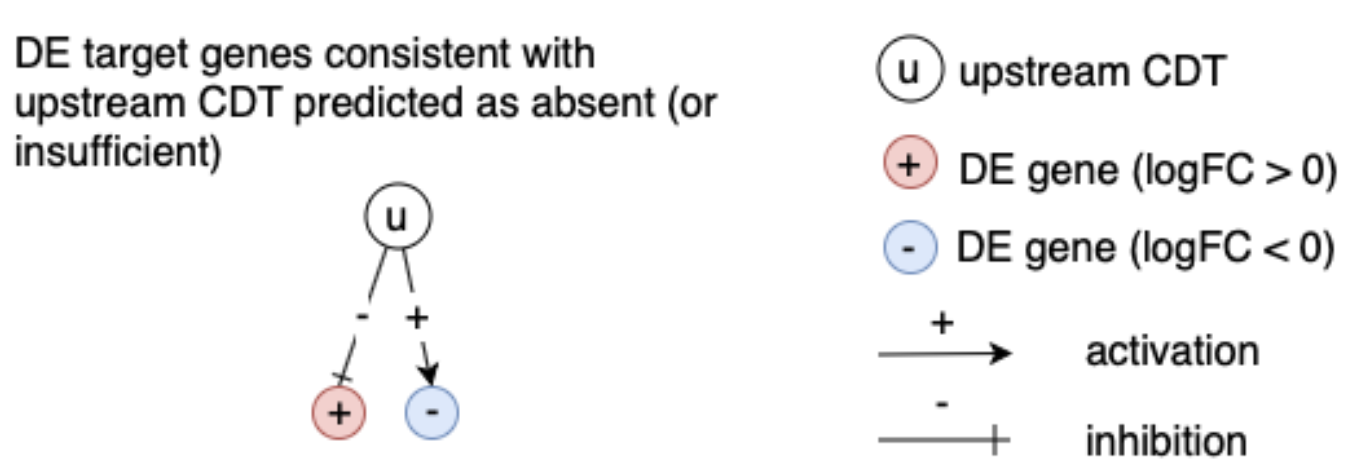
\includegraphics[width=0.6\linewidth]{../Figures/TwoHypotheses.png}
        \caption{A candidate for repurposing would revert the changes of the  observed DE genes. This potential drug \emph{u} would repress the  gene which is up-regulated by the disease (red circle) and would activate the one that is repressed (blue circle). }
        \label{TwoHypotheses}
\end{figure}

\begin{figure}
	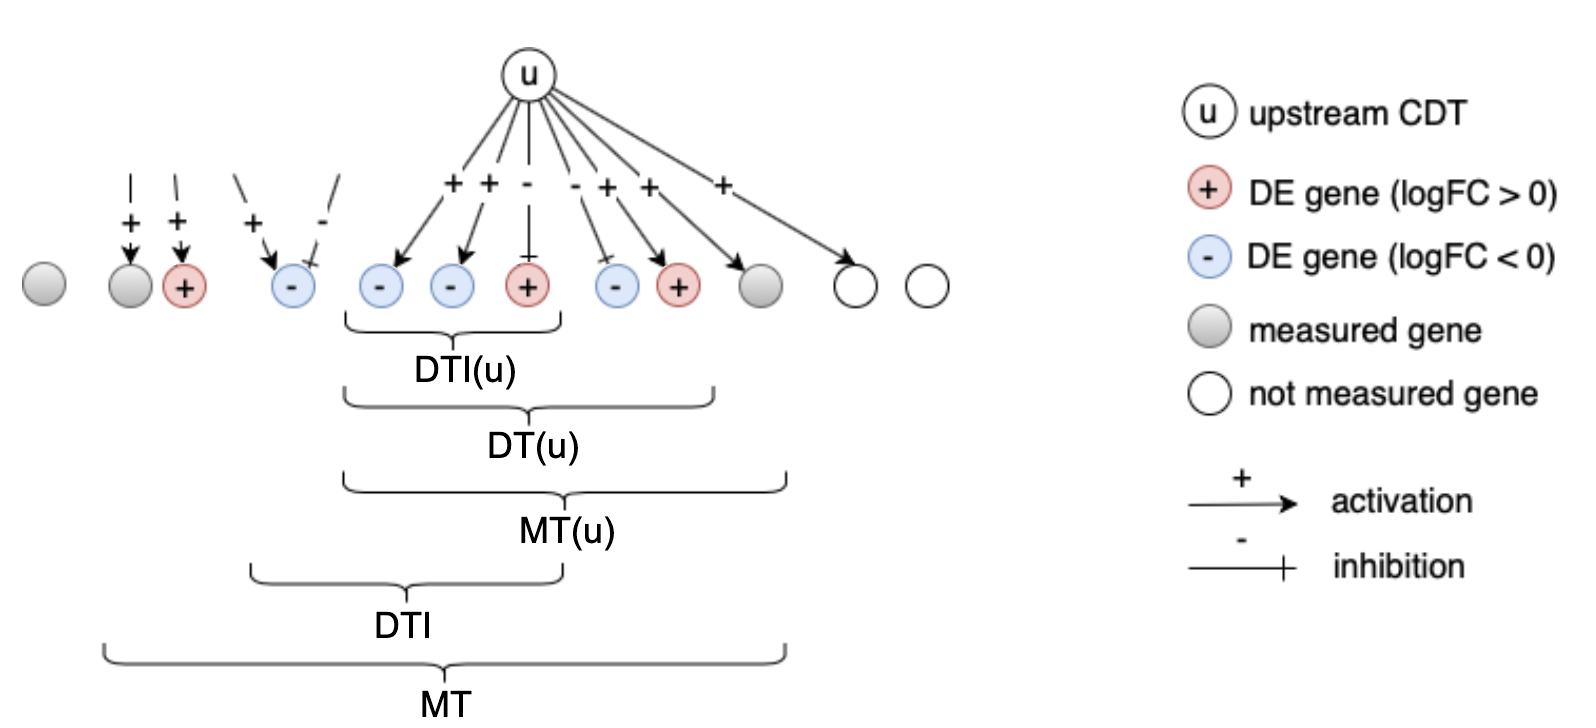
\includegraphics[width=0.9\linewidth]{../Figures/MeasuredGenes.png}
        \caption{The set of all genes includes the set of measured genes that are also targets in the network, or Measured Targets (MT). We define the subset of ``DE Targets consistent with the hypothesis that the CDTs are  insufficient'', DTI. For a selected upstream CDT \emph{u}, we have the set of ``Measured Targets of u'' MT(u), ``Differentially expressed Targets downstream of u'' DT(u), and the set of ``DE targets consistent with the hypothesis that u is insufficient'' DTI(u).}
        \label{MeasuredGenes}
\end{figure}

%\newpage

For the research hypothesis considered, the analysis computes a z-score, $z(u)$, for each CDT $u$, by iterating over the genes that are differentially expressed and immediately downstream of $u$, $DT(u)$: 


\begin{equation}
\label{eq:zscore}
z(u)=\frac{\sum\limits_{g \in DT(u)} sign(e(u,g)) \times sign(g)}{\sqrt{|DT(u)|}}
\end{equation}

where $sign(g)$ is the sign of the DE gene $g$ (1 for up-regulated and -1 for down-regulated), $e(u,g)$ represents an edge from $u$ to $g$,  $sign(e(u,g))$ reflects its type of interaction ($1$ for activation and $-1$ for inhibition), and $|DT(u)|$ represents the number of genes that are differentially expressed and immediately downstream of $u$. 


Under the null hypothesis, the sign of an edge, $sign(e_i)$, and the sign of a gene, $sign(g_i)$, are independent and identically distributed random variables that have either values $-1$ or $1$.  Let $X_i = sign(e_i) \times sign(g_i)$ denote the product of these two variables. Therefore, $X_i$ is also a random variable taking values from $\{-1,1\}$, with the expected value $E[X_i] = \mu = 0$, variance $Var[X_i] = \sigma^2 = 1$. Considering an upstream CDT with $n$ downstream genes ($n = |DT(u)|$), the  average of $n$ samples of $X_i, i \in \{1,...,n\}$ is $\overline{X}_n$.  According to the central limit theorem, the variables $\sqrt{n}(\overline{X}_n - \mu)$ converge  to a normal distribution $N(0,1)$ for large values of $n$. With $\mu = 0$, those variables can be written as:

\begin{equation}
\sqrt{n} \cdot \overline{X}_n = \frac{n \cdot \overline{X}_n} {\sqrt{n}} = \frac{n \cdot \frac{\sum_{i=1}^n X_i}{n}}{\sqrt{n}} = \frac{\sum_{i=1}^n X_i}{\sqrt{n}}
\end{equation}

The numerator is actually the sum of all $n$ samples $X_i$, $\sum{X_i}$, which is also the numerator of equation \ref{eq:zscore}. 
Moreover, we have $n = |DT(u)|$.
Hence, we can conclude that the variable $z(u)$ follows a standard normal distribution, $N(0,1)$. Therefore, we can compute the p-value corresponding to the z-score $P_z$ as the one-tail area under the probability density function for normal distribution.

\textbf{Identifying candidate drugs for repurposing.}
A good candidate for repurposing would revert many of changes observed. This is equivalent  with the research hypothesis that considers the condition is due to a given CDT that is present in insufficient amounts.
We use $P_{abs}$ and $P_z$ to predict upstream CDTs that would revert the measured changes. 
%This hypothesis is also relevant when investigating whether the given phenotype has been impacted by the lack of a given chemical that is necessary for the well-functioning of the organism or cell (e.g. a vitamin deficiency, iron deficiency, etc.). Here, the research hypothesis states that the upstream CDT are insufficient in the condition studied. 
For each upstream CDT $u$, the number of consistent DE genes downstream of $u$, $DTI(u)$, is compared to the number of measured target genes expected to be both consistent and DE just by chance. The uncorrected p-value $P_{abs}$ is computed using the hypergeometric distribution~\cite{DraghiciOT:2003, DraghiciBook:2011}. The analysis combines $P_{abs}$ and $P_z$, using  Fisher's method~\cite{fisher1925statistical}. %where $P_z$ is considered only for significant negative z-scores ($z \leqslant -2$).



\textbf{Clinical Validation.} 
We evaluated the MP protocol with a single pretest, single post-test quasi-experiment from March 12-March 27, 2020 at a 5 hospital health system in Michigan. Patients were compared before and after implementation of the MP protocol on March 20th. The clinical characteristics of the patients are shown in Table~\ref{Supp:clinicalcharacteristics}. 
The primary endpoint was 30 day all-cause mortality.  

\textbf{The methylprednisolone protocol.}  
Patients with PCR confirmed COVID-19 who required 4 liters or more of oxygen per minute on admission, or who had escalating oxygen requirements from baseline, were recommended to receive IV methylprednisolone 0.5 to 1 mg/kg/day in 2 divided doses for 3 days. Patients who required ICU admission were eligible to extend the IV methylprednisolone course to a maximum of 7 days at the discretion of the medical team. Institutional guidelines also recommended hydroxychloroquine 400 mg twice daily for 2 doses on day 1, followed by 200 mg twice daily on days 2--5.

\textbf{Statistical Analysis of clinical data.} Continuous variables were reported as median and interquartile range (IQR) and compared using the Mann-Whitney test or t-test, as appropriate. Categorical data was reported as number and percentage (no., \%) and compared using the chi-squared test or Fisher's exact test, as appropriate. No imputation was made for missing data points. The sample included all eligible consecutive hospitalized patients during the study period. A non-equivalent dependent variable of antibiotic prescribing was utilized to account for potential maturation in treatment. Survival analysis was performed using the Kaplan-Meier method and log-rank test. 


\subsection{Data sources}
This results presented here used data from the Advaita Knowledge Base v 1910, gene ontology data from the GO DB released on April 26, 2019, pathway data from KEGG release 90.0+/05-29, May 2019, miRNA data from MicroCosm Targets version 5, TargetScan version 7.2 (human), miRBase release 22.1, October 2019, interactions from STRING version 11.0 Jan 19, 2019, chemicals, drugs and toxicants from CTD released June 2019, and network data from BioGRID version 3.5.171, March 25th 2019. 


%
%\color{blue} update this part with info on all other data sets included
%\color{black}

The discovery data set used in this analysis, GSE147507, was retrieved from Gene Expression Omnibus (\url{http://www.ncbi.nlm.nih.gov/geo}).  All laboratory work related to this dataset  was done at the Icahn School of Medicine at Mount Sinai  in the tenOever Lab~\cite{Blanco-Melo:2020}. 



\textbf{Gene expression data description} (from the GEO description of this dataset): In this experiment, gene expression data were measured from human lung epithelium (NHBE) and transformed lung alveolar (A549) cells mock treated or infected with SARS-CoV-2 at different multiplicity of infection (MOI) (NHBE: 2 and A549: 0.2). Other independent biological duplicates of A549 cells were mock treated or infected with respiratory syncytial virus A2 strain (MOI 15) or with influenza A virus H1N1 strain (MOI 5). 

\textbf{Cell lines:} Independent biological triplicates of primary human lung epithelium (NHBE) were mock treated (3 samples) or infected with SARS-CoV-2 (3 samples) (USA-WA1/2020), corresponding to series 1 in the data set GSE147507.
%, IAV (A/Puerto Rico/8/1934 (H1N1)), a IAV that lacks the NS1 protein (IAVdNS1) and treated with human interferon-beta. 
Independent biological triplicates of transformed lung alveolar (A549) cells were mock treated or infected with SARS-CoV-2 (USA-WA1/2020) (series 5, 3 controls vs. 3 conditions), RSV (A2 strain) (series 3, 2 controls vs. 2 conditions) or IAV (A/Puerto Rico/8/1934 (H1N1)) (series 4, 2 controls vs. 2 conditions). %\blue{\st{Additionally, independent biological triplicates of transformed lung alveolar (A549) transduced with a vector expressing human ACE2, were also mock treated or infected with SARS-CoV-2 (USA-WA1/2020). Finally transformed lung-derived Calu-3 cells were mock treated or infected with SARS-CoV-2 (USA-WA1/2020).}}

\textbf{COVID-19 patient samples:} Uninfected human lung biopsies were derived from one male (age 72) and one female (age 60) and used as biological replicates. Additionally, lung samples derived from a single male COVID-19 deceased patient (age 74) were processed in technical replicates. These samples are corresponding to series 15 in the data set GSE147507. Experiments using samples from human subjects were conducted in accordance with local regulations and with the approval of the institutional review board at the Icahn School of Medicine at Mount Sinai under protocol HS12-00145.

The initial results obtained from the data above were subsequently confirmed using additional validation data sets, spanning again all  three types of samples: cell lines, tissue cultures, and patient samples. More precisely:  

\textbf{Cell line}: Vero E6 cells either infected with SARS-CoV-2 or mock-infected with three replicates each. The RNA sequencing was performed on the samples 24 hours after infection. The data is available in GEO as the GSE153940~\cite{Riva:2020}.

\textbf{Lung tissue cultures}: Ten lung organoid samples generated from primary lung AT2 cells were either treated SARS-CoV-2 (5 samples) or mock (5 samples). The data is available in GEO as  GSE160435.

\textbf{Intestine tissue cultures}: Intestinal organoids were grown in expansion conditions or differentiation media and either treated with SARS-CoV-2 or treated (2 samples for each condition). The RNA sequencing was performed after 60 hours of infection. The data is available in GEO as GSE149312~\cite{Lamers:2020}.

\textbf{COVID-19 patient samples:} 29 autopsy samples from 8 deceased patients with high viral load were collected to compare with 5 control samples. The data was provided by the Massachusetts General Hospital and Columbia University Irving Medical Center and is available in GEO as GSE150316~\cite{desai2020temporal}.



\subsection{Study limitations}
This study has several limitations as follows. The drugs recommended here are supporting and modulating the immune system response but will not kill the virus and will not prevent infections. They are likely to be useful only for patients with very severe symptoms caused by over-inflammation,  cytokine storm syndrome, etc.  
The use of these drugs has to be decided in the context of the entire clinical profile of the patient including the clinical stage~\cite{siddiqi2020covid}, co-morbidities, other risk factors, etc.


Highly significant p-values indicate that the result is extremely unlikely to be due to random chance, but does not necessarily speak to the clinical significance of the finding. 

The drugs that were found not to have the potential to revert the gene expression changes triggered by SARS-CoV2 may have other beneficial effects (e.g. antiviral), and may be useful in earlier disease stages. 




The  A549 cell line  is a cancer cell line. In this cell line many phenomena may be very different than in the epithelial tissue in the normal lung. This was taken into consideration by basing most of the analysis on the other data. Nevertheless, all the results coming from the A549 cell line should be considered in the light of the fact that these are not normal cells. 

The Vero cell line was initially isolated from kidney epithelial cells extracted from an African green monkey and are interferon-deficient. Unlike normal mammalian cells, they do not secrete interferon alpha or beta when infected by viruses. However, they still have the interferon-alpha/beta receptor, so they respond normally when recombinant interferon is added to their culture media. These characteristics of this cell line may influence the results obtained with them. 

Given the pandemic nature of the disease a pragmatic quasi-experimental design was used for the clinical study. The potential for regression to the mean and maturation is an inherent limitation to all quasi-experiments. 
After March 16, 2020 some of the pre-steroid group experienced delayed diagnosis and treatment due to the adoption of rapid on-site RT-PCR testing for SARS-CoV-2. However, the observed association was unchanged in the sensitivity analysis.  A non-equivalent dependent variable, empiric antibiotic therapy for pneumonia, suggested no difference in management of COVID-19. 
Some of the pre-MP protocol group received MP after initiation of the updated COVID-19 institutional treatment protocol.  MP initiated in this group were started  later. Additionally, guideline adherence in the MP  group was not universal. 

Although the group treated with MP had a lower death rate, it also started with a lower rate of co-morbidities in 8/9 conditions (Table~\ref{Supp:clinicalcharacteristics}). Even though none of these differences have a statistically significant impact on the survival analysis, they may influence the results. 


\subsection{Henry Ford Hospital Division of Infectious Diseases Management and Treatment of COVID-19 Cases Guideline}


All confirmed COVID-19 inpatients require Infectious Diseases consultation for management. For testing recommendations, please refer to SARS-CoV-2 (COVID-19) Testing Criteria from HFHS infection prevention and control. \url{https://onehenry.hfhs.org/documentcenter/Business%20Units%20%20Departments/SARS-CoV-2%20(COVID-19)%20Testing%20criteria%20v3.12.2020.pdf} 

At the time this  study was performed, there were \textbf{no FDA approved therapies to treat COVID-19}. Some medications have demonstrated in vitro, animal, or very limited clinical safety and efficacy data in other coronaviruses (e.g. SARS and MERS). The Division of Infectious Diseases is coordinating research/compassionate use remdesivir. The below treatments should be started immediately once COVID test is positive (when indicated), pending remdesivir availability.  Preemptively starting COVID medications prior to return of test results is not recommended due to limited medication supply unless there is high suspicion based upon clinical judgement and patient characteristics.  These guidelines are interim recommendations and may change according to drug availability and new data published. Supportive care and infection control measures are indicated for all hospitalized patients.

\textbf{Initial labs for all inpatients} (see below for ongoing treatment monitoring): 
\begin{itemize}
\item Suspected or confirmed patients: CBC with differential, BMP, magnesium, ferritin, liver profile, bilirubin, total, procalcitonin, CPK, D-dimer, CRP, LDH, high sensitivity troponin
\item Draw upon admission to ICU: Triglyceride, IL-6, DIC panel (in addition to labs listed above if not previously ordered)
\item Baseline EKG
\end{itemize}

\textbf{Monitoring parameters:}
\begin{itemize}
\item Hydroxychloroquine: Cardiotoxicity, Torsade de Pointes, depression, psychosis. Maintain potassium at least 4 mEq/L, and magnesium at least 2 mEq/L. \textbf{Refer to QT monitoring appendix.} 
\item Remdesivir: Phlebitis, Constipation, Nausea, Headache, Bruising, Liver Function test abnormalities. Obtain daily BMP and LFTs. 
\end{itemize}




The treatments used for the COVID-19 patients are shown in Figure~\ref{Supp:TreatmentCovidPatient}.



\begin{figure*}
\centering
	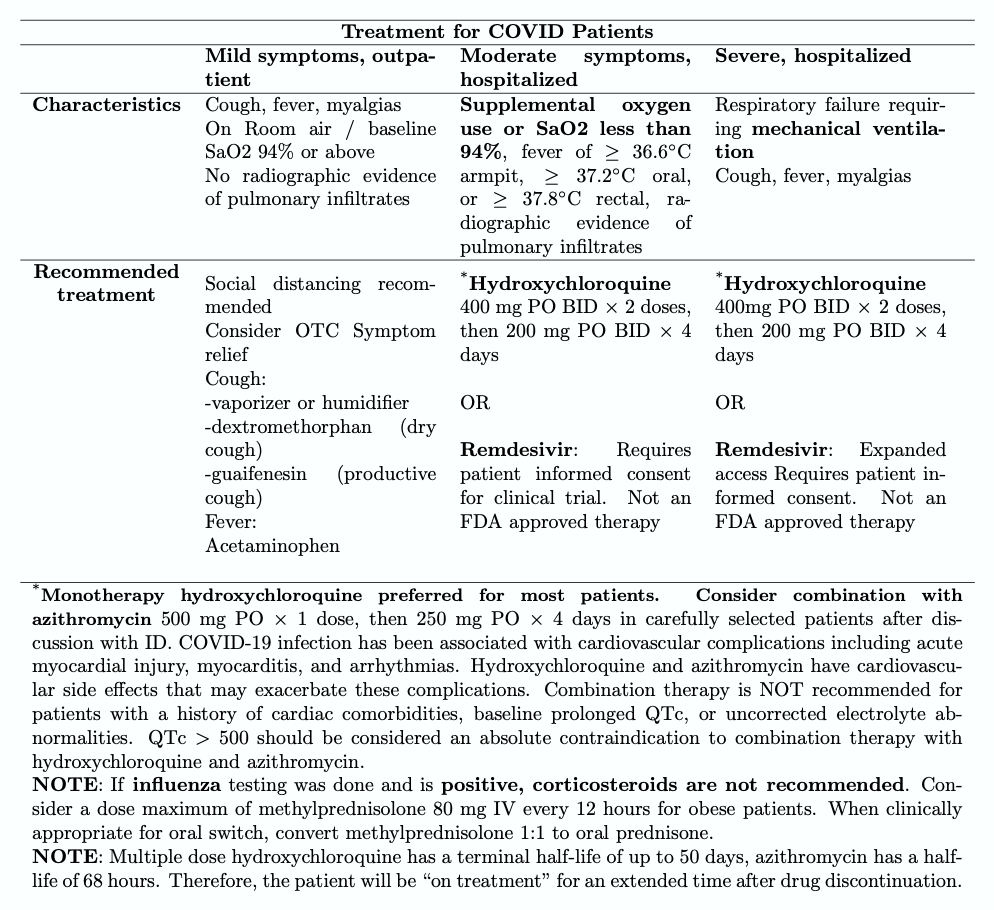
\includegraphics[width=0.9\linewidth]{../Figures/TreatmentCOVIDPatients.png}
    \caption{ Treatments use for COVID patients.}
        \label{Supp:TreatmentCovidPatient}
\end{figure*}










